\section{Using functions with different numbers of parameters} % 5 pages
\label{sec:correction}

\subsection{Corrections to the likelihood}
\label{sec:correction:corrections}

The \nll calculated from the fit of a function to a dataset is purely a measure
of the agreement of the function and the data; the
number of parameters $N_{\rm par}$
used in the function has no impact. Hence, at least for nested families of
functions (such as polynomials of varying order), then the lowest \nll will
always be given by the highest order considered.
Because this function also has the
largest number of parameters, it will generally have the largest statistical
error and hence widest profiled \nll curve.
Hence, simply using the \nll values
without any ``penalty'' for the number of parameters would effectively
always result in the minimum envelope being mainly defined by the highest
order function considered. It would also mean there is no ``natural'' way to know when
to stop considering yet higher order functions. However, decisions based
on quantities, such as an F-test~\cite{ref:ftest},
are standardly used to determine when higher order functions in
a family can be ignored. Hence, when using functions with different
numbers of parameters, it seems necessary to have some correction to the \nll
value to account for this difference in number.

The idea is therefore to compare \nll values,
correcting for the differing number of parameters
(or equivalently differing number of degrees of freedom) in
the fit functions. Specifically here, where applied, the correction is
done so as to get a value equivalent to a function with no parameters, so
the number of degrees of freedom is the number of bins $N_{\rm bin}$ used.
Two methods were considered, based on the
$\chi^2$ p-value and the Akaike information
criterion~\cite{ref:correction:akaike}.
\begin{enumerate}
\item %[p-value]
For a binned fit using the expression for the \nll ratio
for each bin specified in equation~\ref{eqn:introduction:def2NLL}, then for
the large statistics case, the \nll becomes equivalent to a $\chi^2$ for the
fit. In this case, it is meaningful to find the p-value of the $\chi^2$ value,
which also depends on the number of degrees of freedom.
A new $\chi^{\prime 2}$
value can now be obtained, namely that which would give the same p-value but
with a different number of degrees of freedom,
equal to the number of bins.
Explicitly, the p-value $p$ is the upper
tail integral of the $\chi^2$ probability
distribution which we write as
\begin{displaymath}
p = F(\chi^2,N_{\mathrm{bin}}-N_{\mathrm{par}})\qquad\mathrm{so}\qquad
\chi^2 = F^{-1}(p,N_{\mathrm{bin}}-N_{\mathrm{par}}),
\end{displaymath}
Hence, the new $\chi^{\prime 2}$ which gives the same p-value with
$N_{\rm bin}$ degrees of freedom is given by
\begin{displaymath}
\chi^{\prime 2} = F^{-1}(p,N_{\rm bin})
\end{displaymath}
and the corrected \nll is then given by
\begin{displaymath}
\Lambda_{\mathrm{corr}} = \textrm{\nll} + (\chi^{\prime 2} - \chi^2).
\end{displaymath}
In the work presented here,
this correction was applied even though some bins in the fits
have lower statistics,
such that the \nll is not a particularly good approximation to the $\chi^2$.

Besides being a function of the number of bins and parameters,
the size of the correction $\chi^{\prime 2} - \chi^2$
depends on the original fit quality
(or equivalently p-value). Figure~\ref{fig:correction:DeltaChiSq}
shows examples of the size of the correction as a function of the
fit p-value, when correcting for various numbers of parameters.
The correction is monotonically decreasing as the p-value gets larger.
Hence, when correcting the profile likelihood curve, the fits further away from
the best fit minimum will get a larger correction. Hence, the profile curve
becomes steeper, which could in principle affect the coverage, even if
only considering one fit function.
%Figure~\ref{fig:parameters:pvalue} shows the effect of the correction
%for the power-law fit on the profile
%(shown uncorrected in figure~\ref{fig:nuisance:powfit})
%and on the Neymann fraction
%(shown uncorrected in figure~\ref{fig:nuisance:powfraction}).
%In both cases, the effect of the correction is almost negligible
%in practice.
However, it can be seen that the correction is approximately given by
\begin{displaymath}
\chi^{\prime 2} - \chi^2 \approx N_{\rm par},
\qquad{\rm so}\qquad
\Lambda_{\mathrm{corr}} \approx \textrm{\nll} + N_{\rm par}
\end{displaymath}
for the central range of p-values. This approximation means the
$\Lambda_{\mathrm{corr}}$ shape, and hence coverage, is unchanged when considering one function alone. Both the
exact p-value
correction and the $N_{\rm par}$ approximate correction are studied in this paper.
%
\begin{figure}[tbp]
\centering
 \subfigure[]{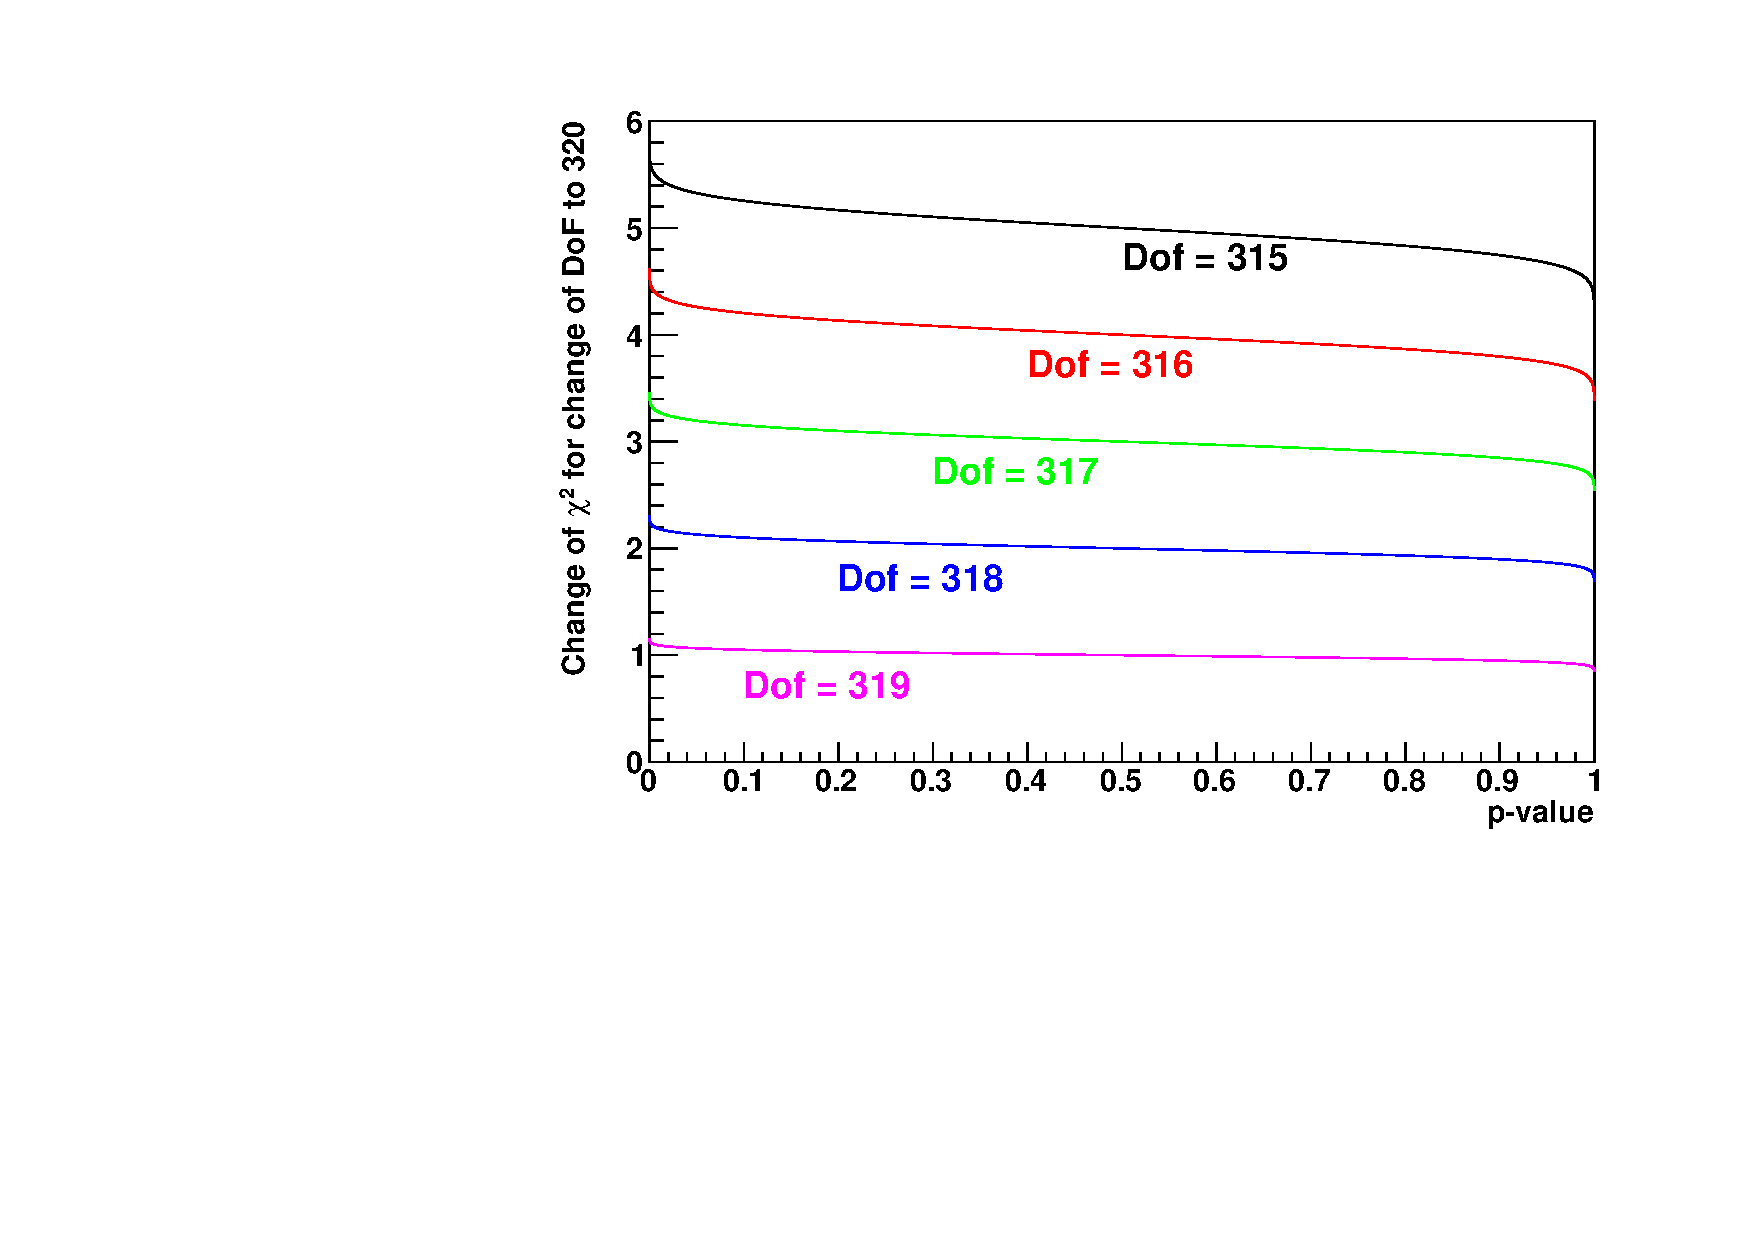
\includegraphics[width=0.46\textwidth]{correction/DeltaChiSq1.pdf}
\label{fig:correction:DeltaChiSq:a}}
 \subfigure[]{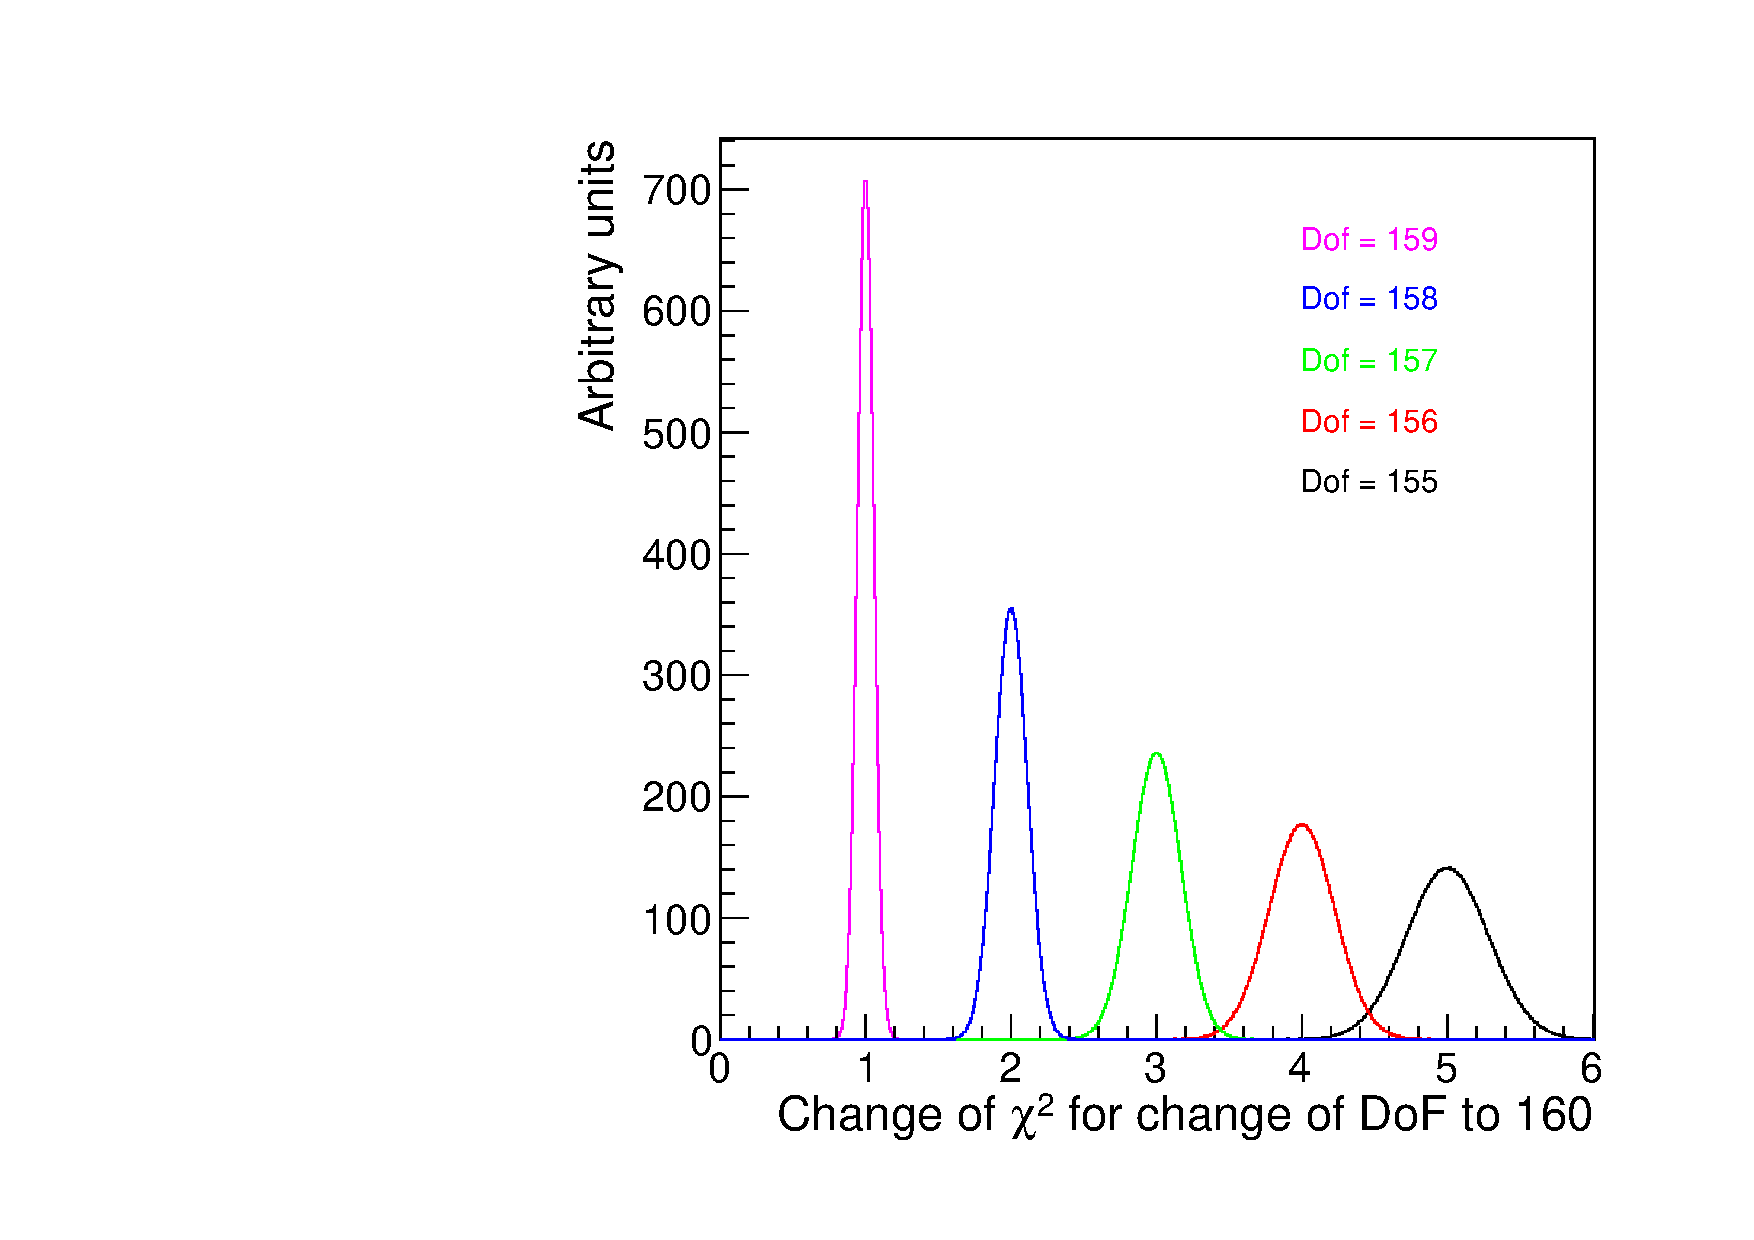
\includegraphics[width=0.46\textwidth]{correction/DeltaChiSq2.pdf}
\label{fig:correction:DeltaChiSq:b}}
\caption{Change of $\chi^2$ when correcting for between one and five parameters
in a fit with 160 bins. (a) The change to the $\chi^2$ as a function of the
original p-value. (b) The distribution of the change of
the $\chi^2$ assuming a flat p-value distribution.}
\label{fig:correction:DeltaChiSq}
\end{figure}


\item %[Akaike]
The basic Akaike formula for very large sample sizes is
\begin{displaymath}
\Lambda_{\mathrm{corr}} = \textrm{\nll} + 2N_{\rm par},
\end{displaymath}
%The resulting value of $A$ is considered here as the corrected \nll,
so the correction is simply $ 2N_{\rm par}$ and
hence is twice as big as the approximate p-value correction.
For finite samples, then it is modified to
\begin{displaymath}
\Lambda_{\mathrm{corr}}
= \textrm{\nll} + 2N_{\rm par}  + \frac{2N_{\rm par}(N_{\rm par}+1)}{n-(N_{\rm par}+1)}
= \textrm{\nll} + \frac{2N_{\rm par}}{1-(N_{\rm par}+1)/n},
\end{displaymath}
where $n$ is the sample size, i.e.~the number of bins (for a binned likelihood
fit) or events (for an unbinned likelihood fit). For large $n$, the original
formula is clearly regained.
Also the correction does not depend on the \nll value and
so is a simple shift of
the whole profile curve, without changing its shape.
Hence, it also has no effect on coverage when considering one function alone.
\end{enumerate}

\subsection{Function definitions}
\label{sec:correction:functions}
The fit functions which were used are the two-parameter functions listed in
Section~\ref{sec:functions:function} and higher order generalisations of
these. Specifically, these are
\begin{enumerate}
\item
%``Power law sum''; $f(x) = \sum_{i=0}^N p^{a}_{i} x^{p^{b}_{i+1}}$.
``Power law sum''; $f(x) = \sum_{i=0}^N p_{2i} x^{p_{2i+1}} = p_{0}x^{p_{1}} + p_{2}x^{p_{3}} + p_{4}x^{p_{5}}+\cdots$.
\item
%``Exponential sum''; $f(x) = \sum_{i=0}^N p^{a}_{i} e^{p^{b}_{i+1}x}$.
``Exponential sum''; $f(x) = \sum_{i=0}^N p_{2i} e^{p_{2i+1}x} = p_{0} e^{p_{1}x} + p_{2} e^{p_{3}x} + p_{4} e^{p_{5}x}+\cdots$.
\item
``Laurent series''; $f(x) = \sum_{i=0}^N p_i/x^{n_i}$.
\item
``Polynomial''; $f(x) = \sum_{i=0}^N p_i x^i$.
\end{enumerate}
The Laurent function values of $n_{i}$ used for $i=0,1,2,3,4,5\dots$ are
$n_{i}=4,5,3,6,2,7\dots$, meaning they are grouped around the original
two $n_{i}$ values of 4 and 5 as used throughout Section~\ref{sec:functions}.
Note the power law and exponential functions can only have even numbers of
parameters, i.e.~$N_{\rm par}=2N$, while the Laurent and polynomial functions
can have both even and odd numbers, i.e.~$N_{\rm par}=N$.


\subsection{Example case}
\label{sec:correction:example}

The functions listed above were fit to the original dataset for values of
$2 \le N_{\rm par} \le 6$; this resulted in three fits for the power law and
exponential functions, and five fits for the Laurent and polynomial functions.
This range was chosen for practical purposes as these functions gave reasonable
fits, without requiring larger numbers of parameters.
The profile curves from the fits of these functions are shown in
figures~\ref{fig:correction:profiles-no},~\ref{fig:correction:profiles-pval} and~\ref{fig:correction:profiles-akaike} where results for three different
corrections to \nll have been shown, namely no correction, the approximate
p-value correction, and the Akaike correction respectively.
These figures also show the 68.3\% and
95.4\% confidence intervals which would be determined from the
profile envelope. 

Consider the example case of the approximate p-value correction,
i.e.~correcting by one unit per background function parameter,
which is shown
in figure~\ref{fig:correction:profiles-pval}.
For this case, the lowest corrected \nll value is still given by the
two-parameter power law function and so gives an identical central value
to that described in Section~\ref{sec:functions:example}. The lowest corrected
\nll value for $\mu < 0.55$ is also again given by the two-parameter exponential
function, also as for the previous case.
Indeed, comparison with figure~\ref{fig:functions:profiles} shows that the
minimum values of the corrected \nll for low $\mu$
are simply two units larger here than in that figure.
However, for $1.48 < \mu < 1.68$,
the $N_{\rm par}=5$ polynomial is the lowest function in the profile,
while for $\mu > 1.68$,
the $N_{\rm par}=6$ polynomial is lowest.
Hence, the envelope is formed from four different functions in this
case. 
The 68.3\% region is identical to that found using
just the two-parameter functions (see Section~\ref{sec:functions:example}), but
when including higher order functions, the 95.4\% confidence interval
on $\mu$ is $-0.18 < \mu < 2.11$,
i.e.~it is extended to higher $\mu$
due to the influence of the higher order polynomial functions providing a
reasonable description of the data.
%The central value is unchanged since the lowest order power law
%best desribes the data when including a penalty for using additional parameters in the fit.
%
\begin{figure}[tbp]
\centering
\subfigure[]{
 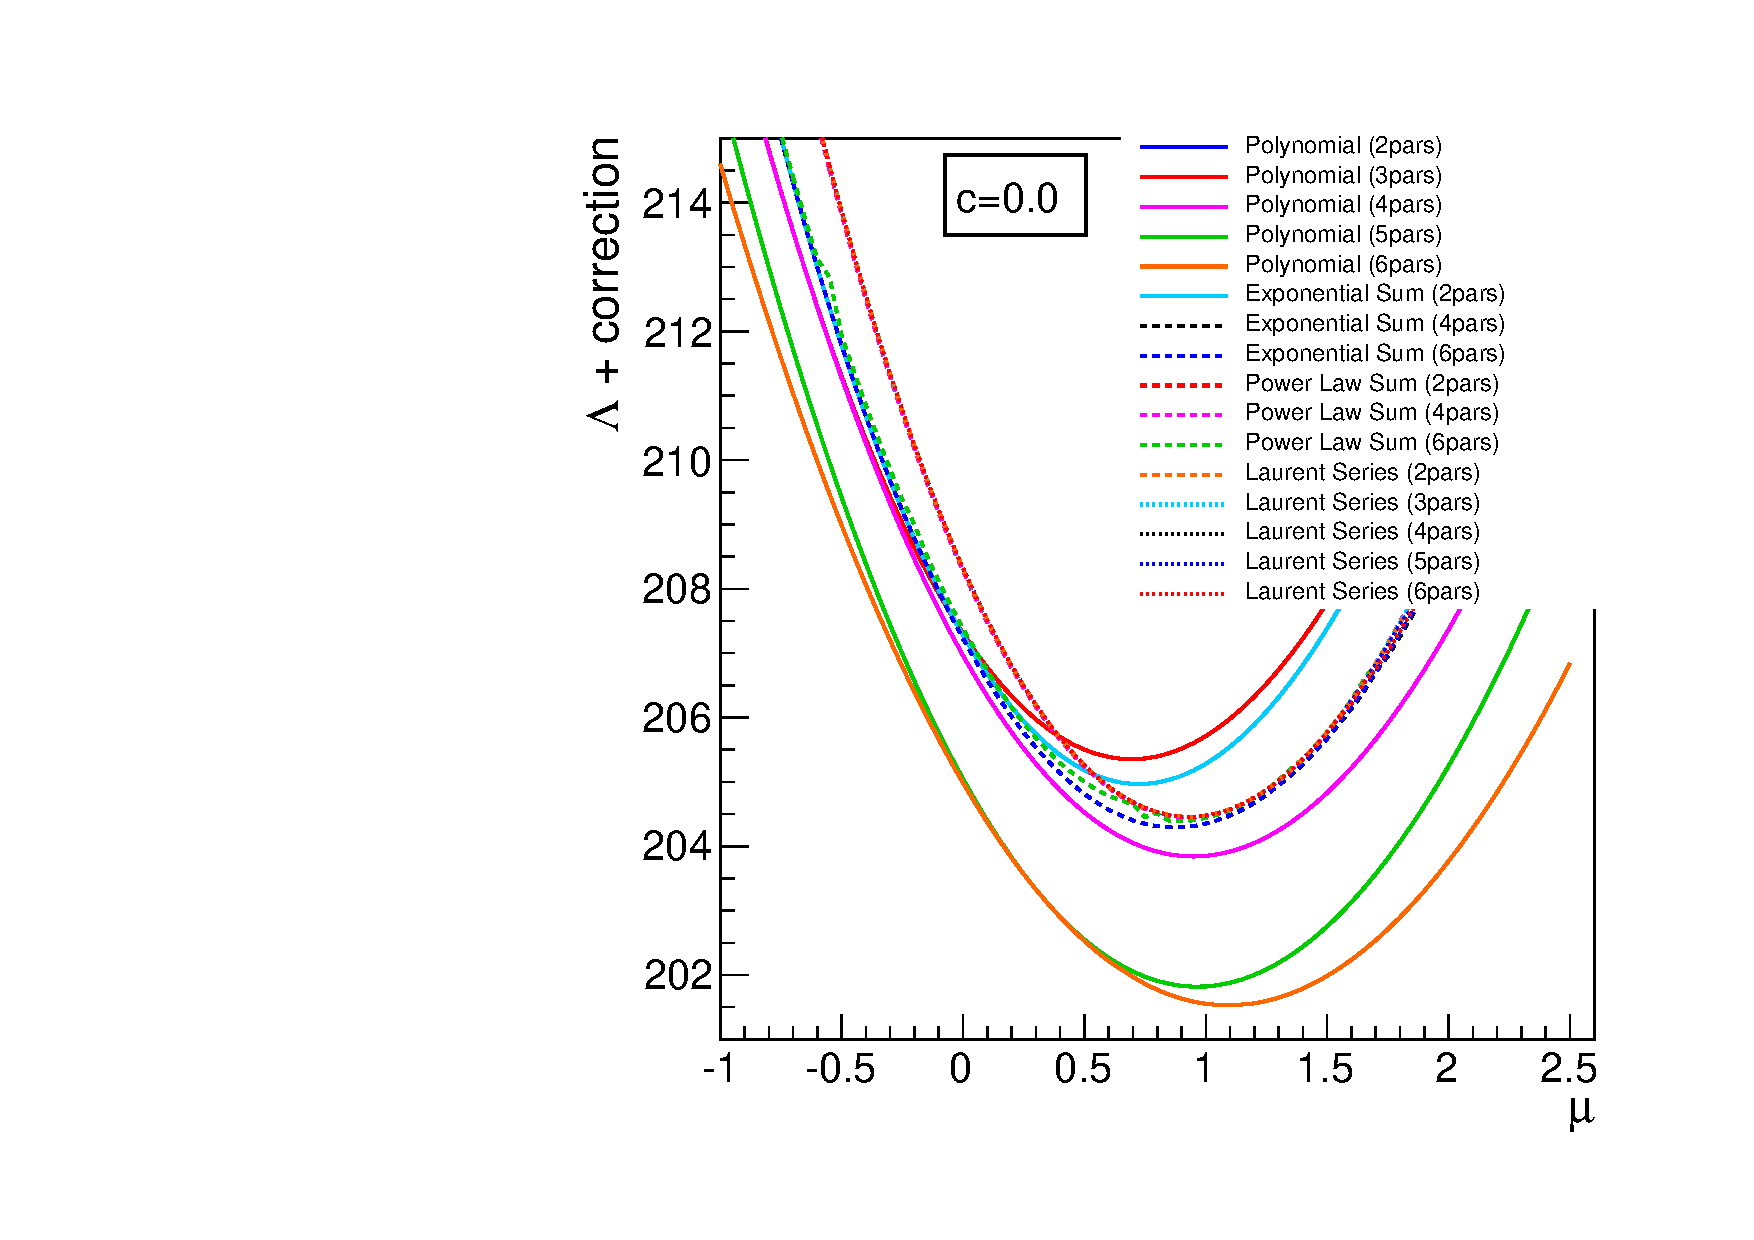
\includegraphics[width=0.46\textwidth]{{correction/ProfilesAllOrders0.0}.pdf}
 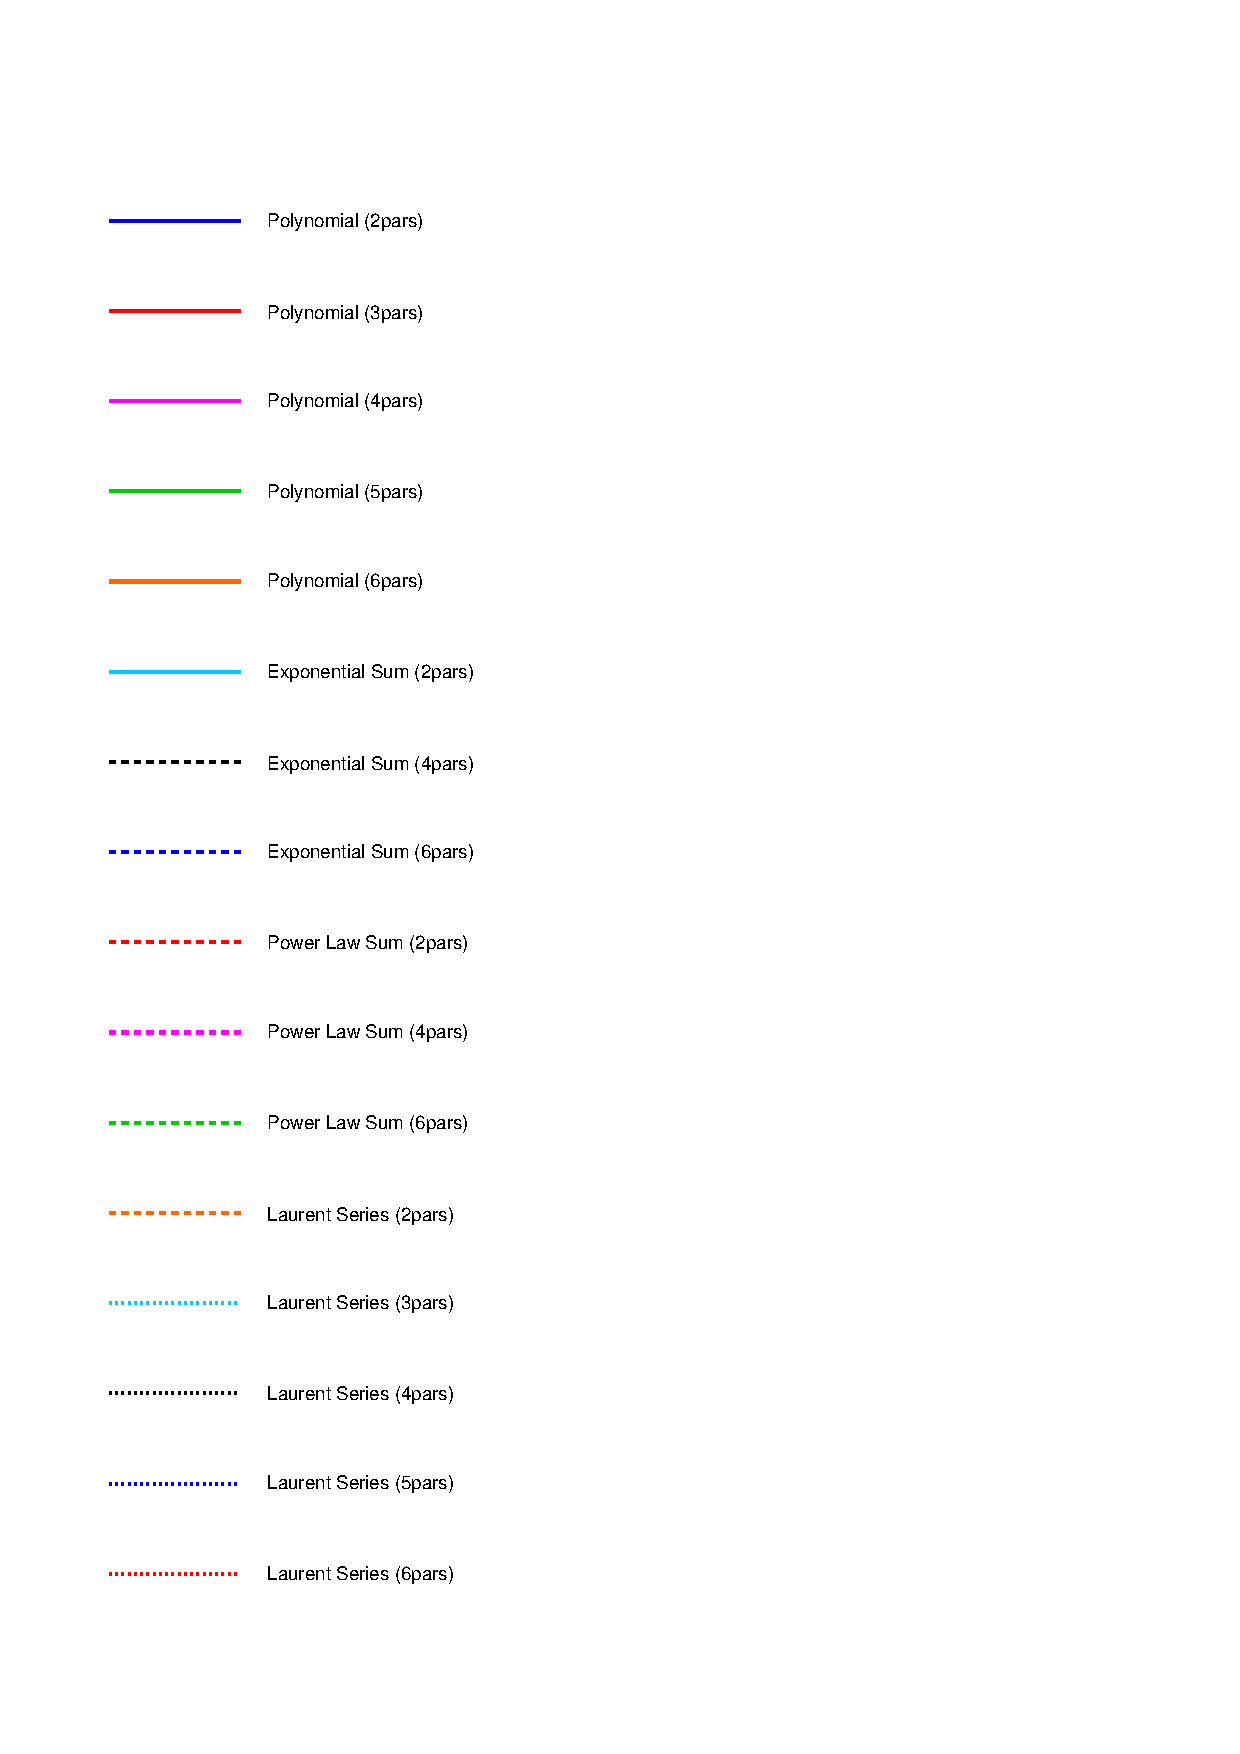
\includegraphics[width=0.46\textwidth]{{correction/AllFunctionsLegend}.pdf}
\label{fig:correction:profiles-no:a}
}
\subfigure[]{
 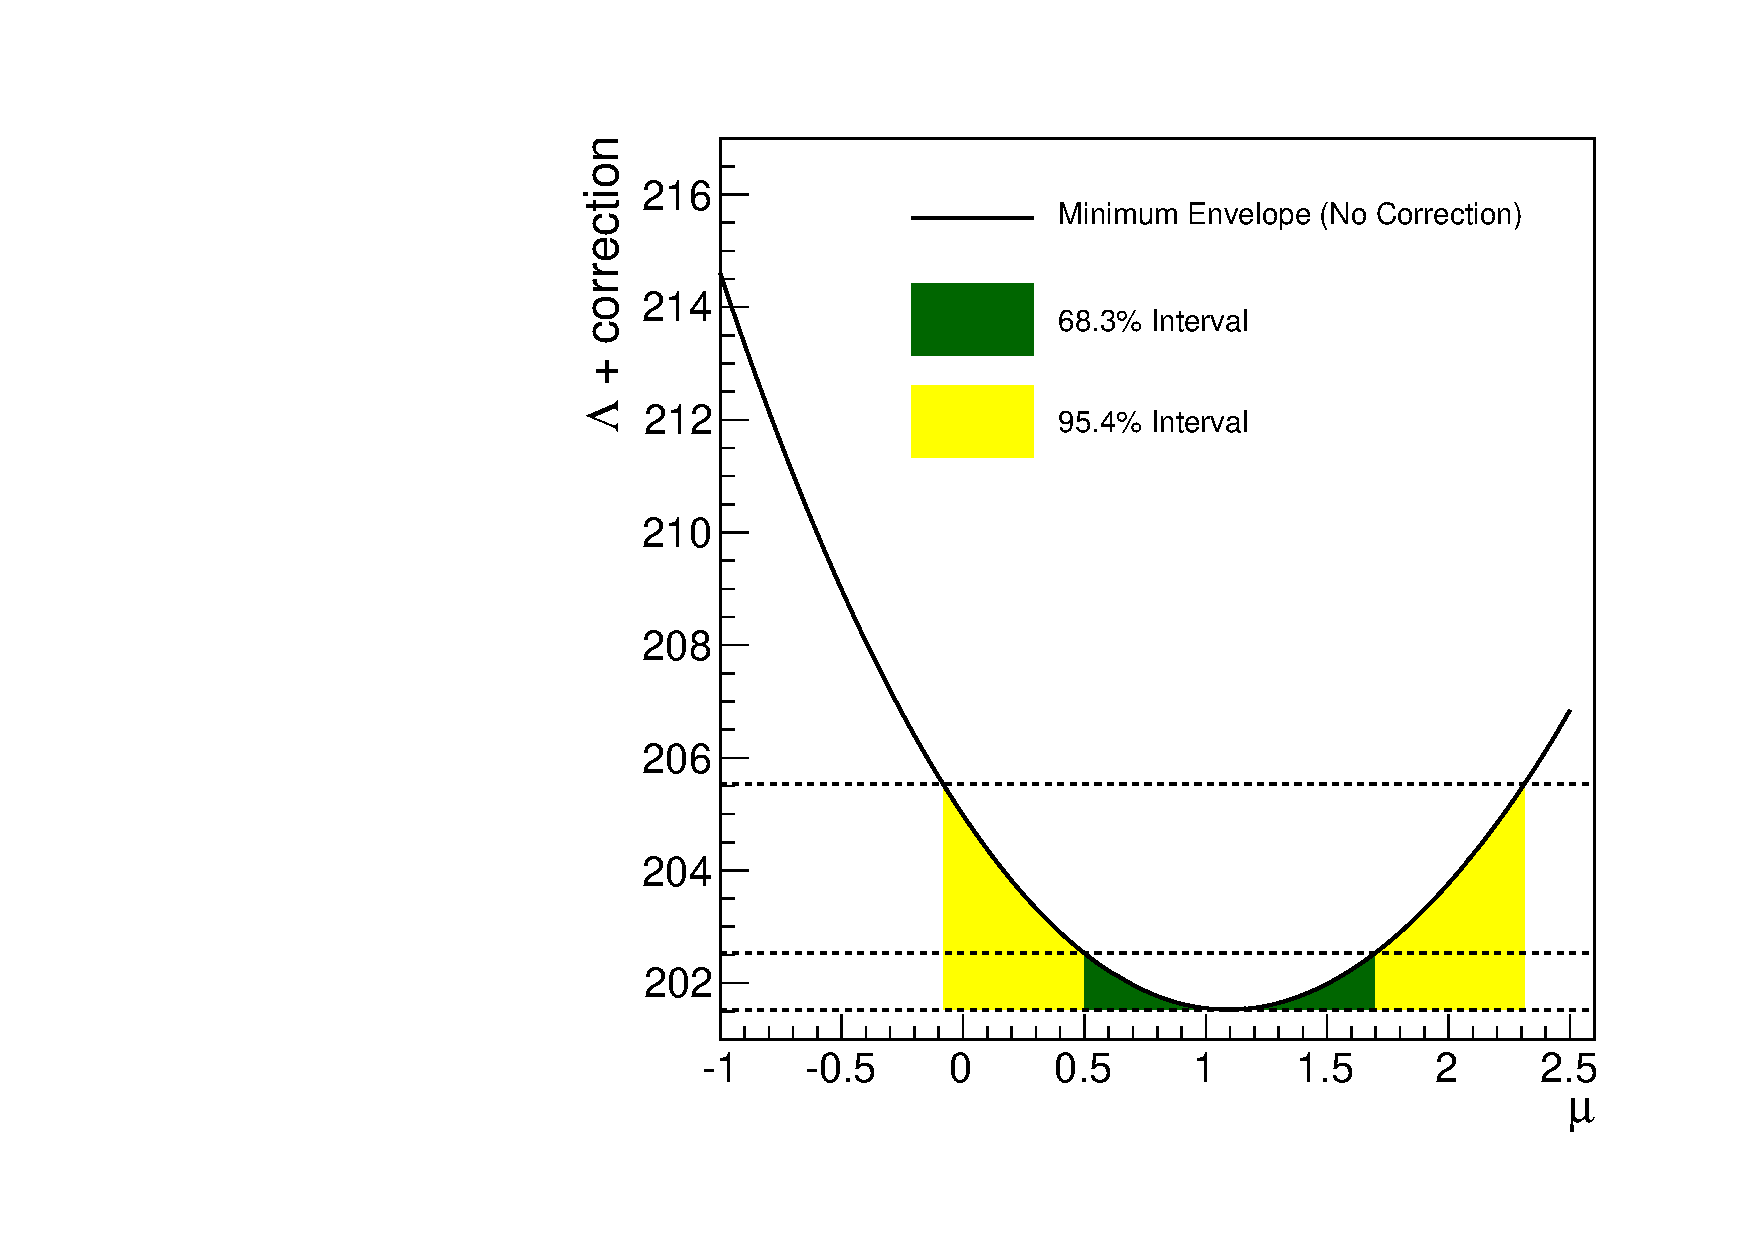
\includegraphics[width=0.46\textwidth]{{correction/EnvelopeAllOrders0.0}.pdf}
\label{fig:correction:profiles-no:b}
}
\caption{(a) Profiled \nll curves for all of the functions considered. The \nll value for each profile curve has not been corrected. The labels indicate the function and the value of $N_{\rm par}$. (b) Minimum envelope of the functions. The \nll scan when only considering the best fit function is drawn in red, although this is completely obscured by the envelope curve in this case.}
\label{fig:correction:profiles-no}
\end{figure}

\begin{figure}[tbp]
\centering
\subfigure[]{
 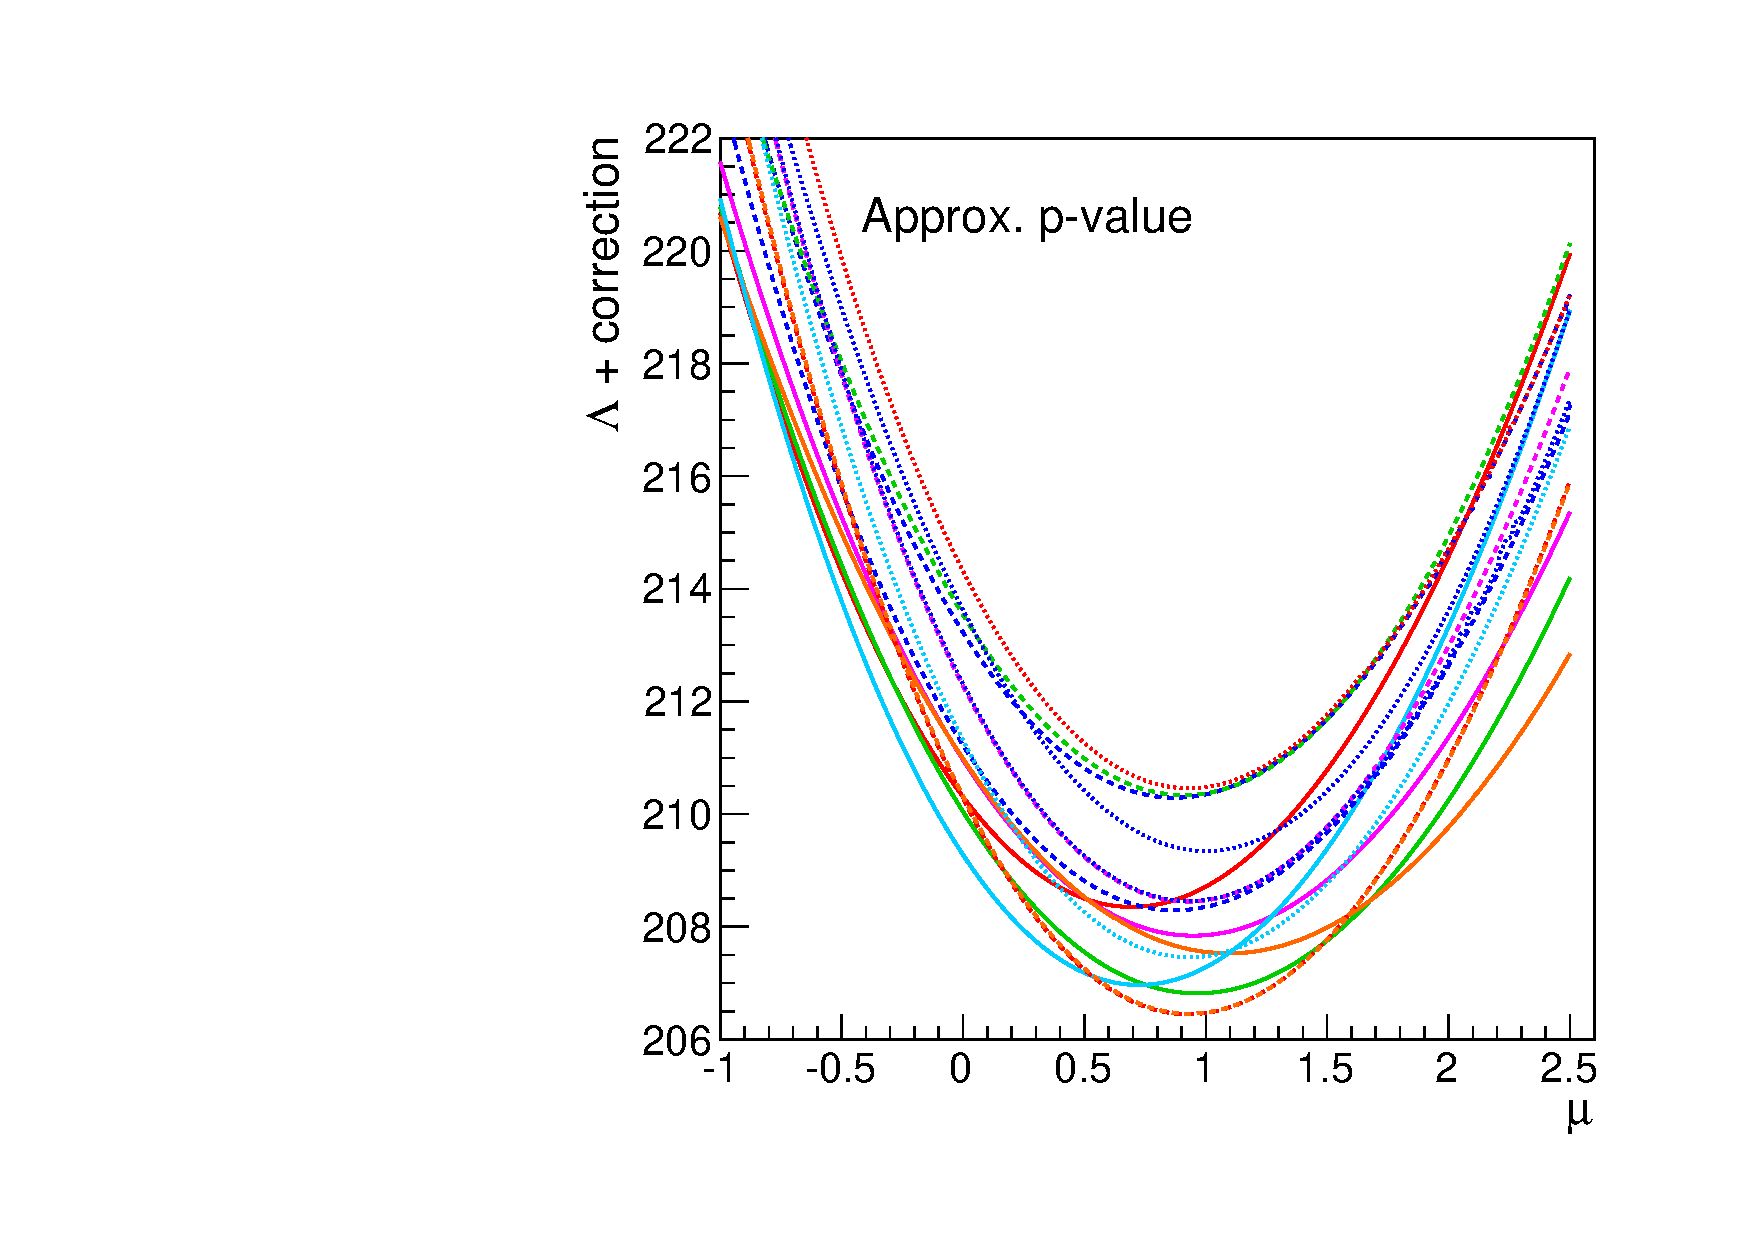
\includegraphics[width=0.46\textwidth]{{correction/ProfilesAllOrders1.0}.pdf}
 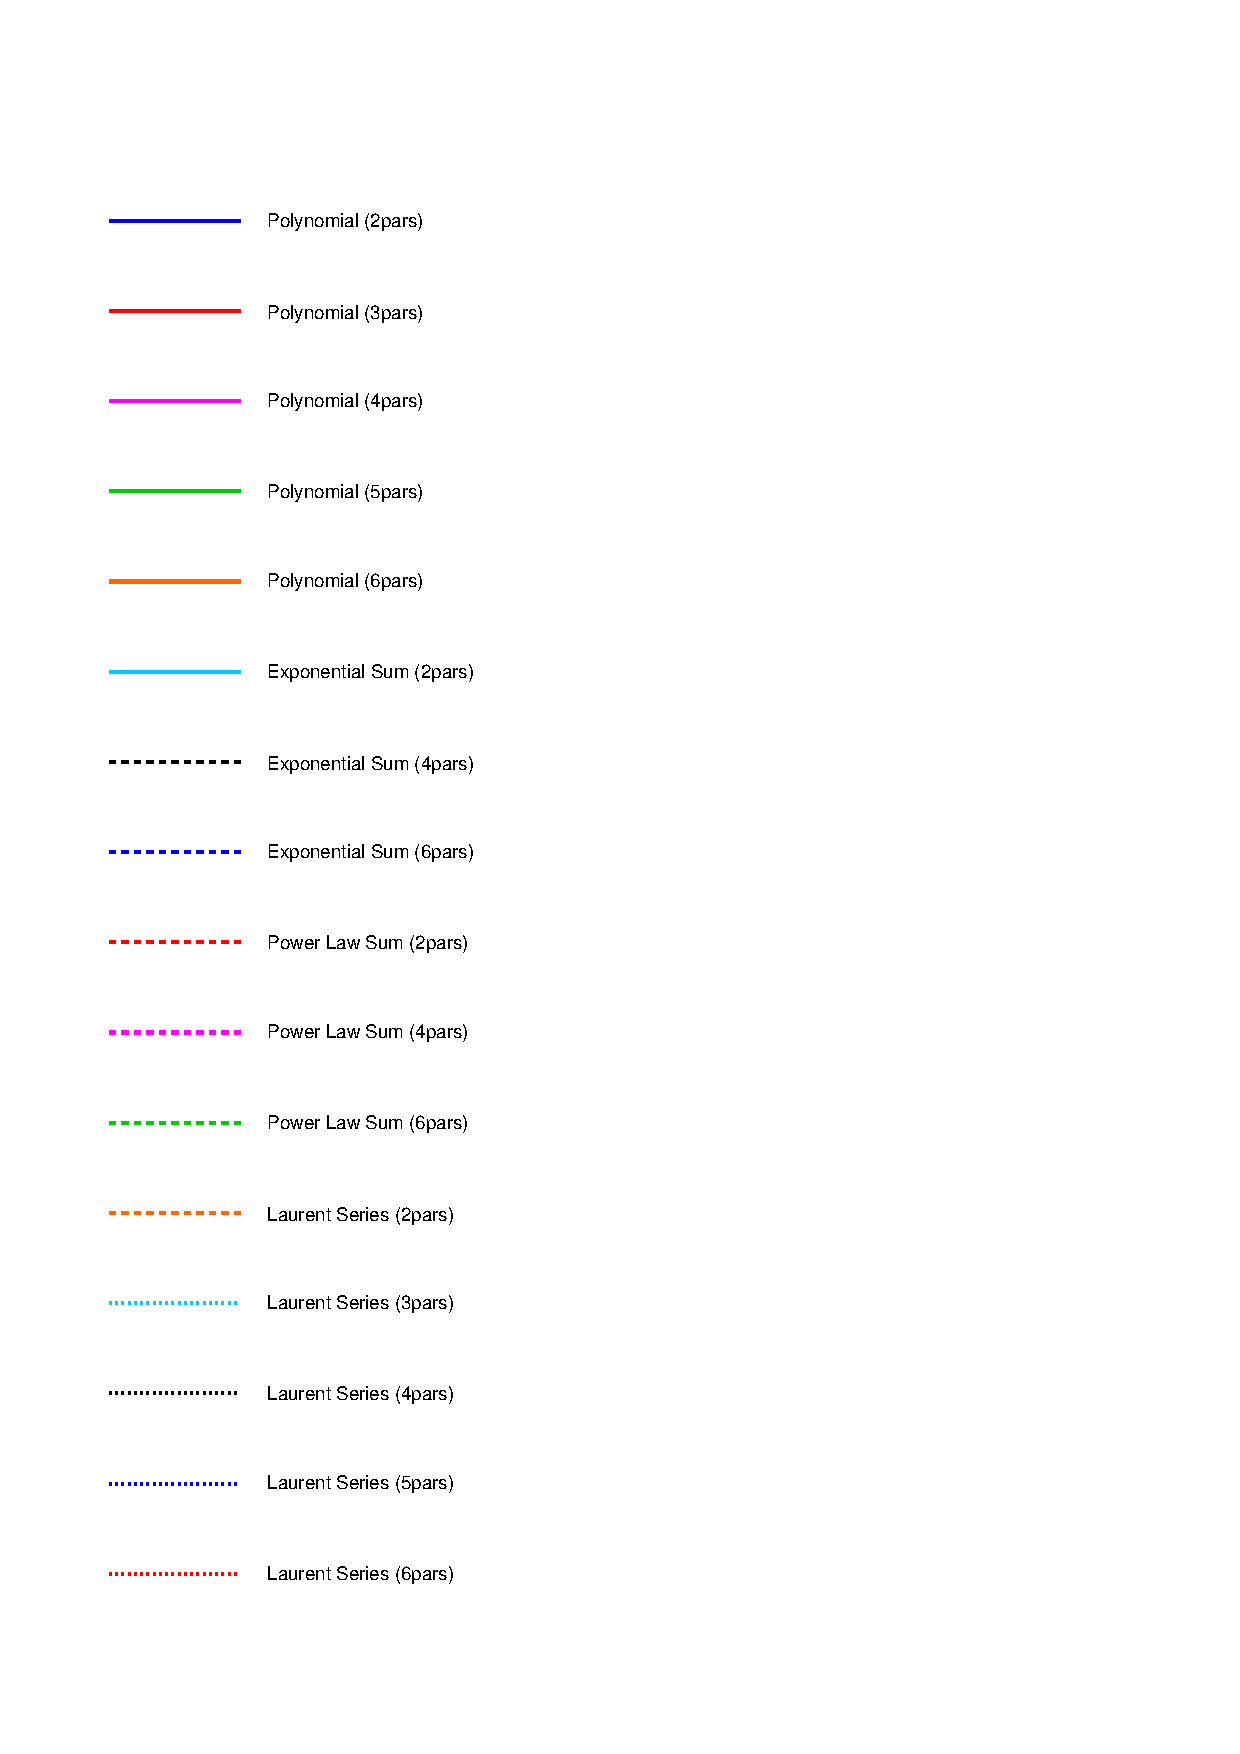
\includegraphics[width=0.46\textwidth]{{correction/AllFunctionsLegend}.pdf}
\label{fig:correction:profiles-pval:a}
}
\subfigure[]{
 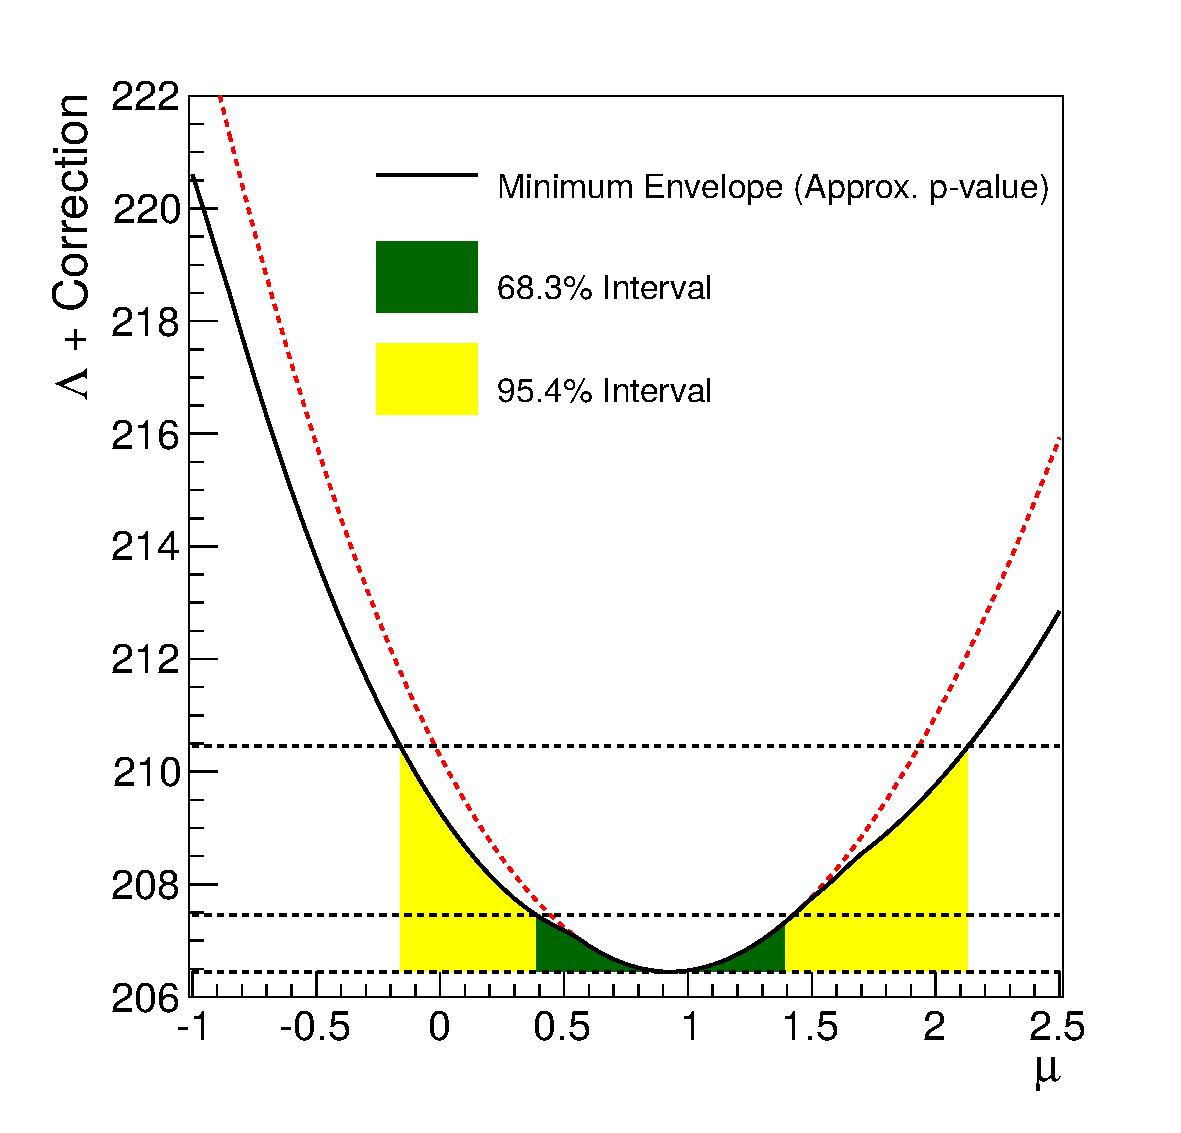
\includegraphics[width=0.46\textwidth]{{correction/EnvelopeAllOrders1.0}.pdf}
\label{fig:correction:profiles-pval:b}
}
\caption{(a) Profiled \nll curves for all of the functions considered. The \nll value for each profile curve has been corrected using the approximate p-value correction of 1 per background parameter. The labels indicate the function and the value of $N_{\rm par}$. (b) Minimum envelope of the functions after applying a correction of 1 per background parameter to each \nll curve. The \nll scan when only considering the best fit function is shown in red.}
\label{fig:correction:profiles-pval}
\end{figure}

\begin{figure}[tbp]
\centering
\subfigure[]{
 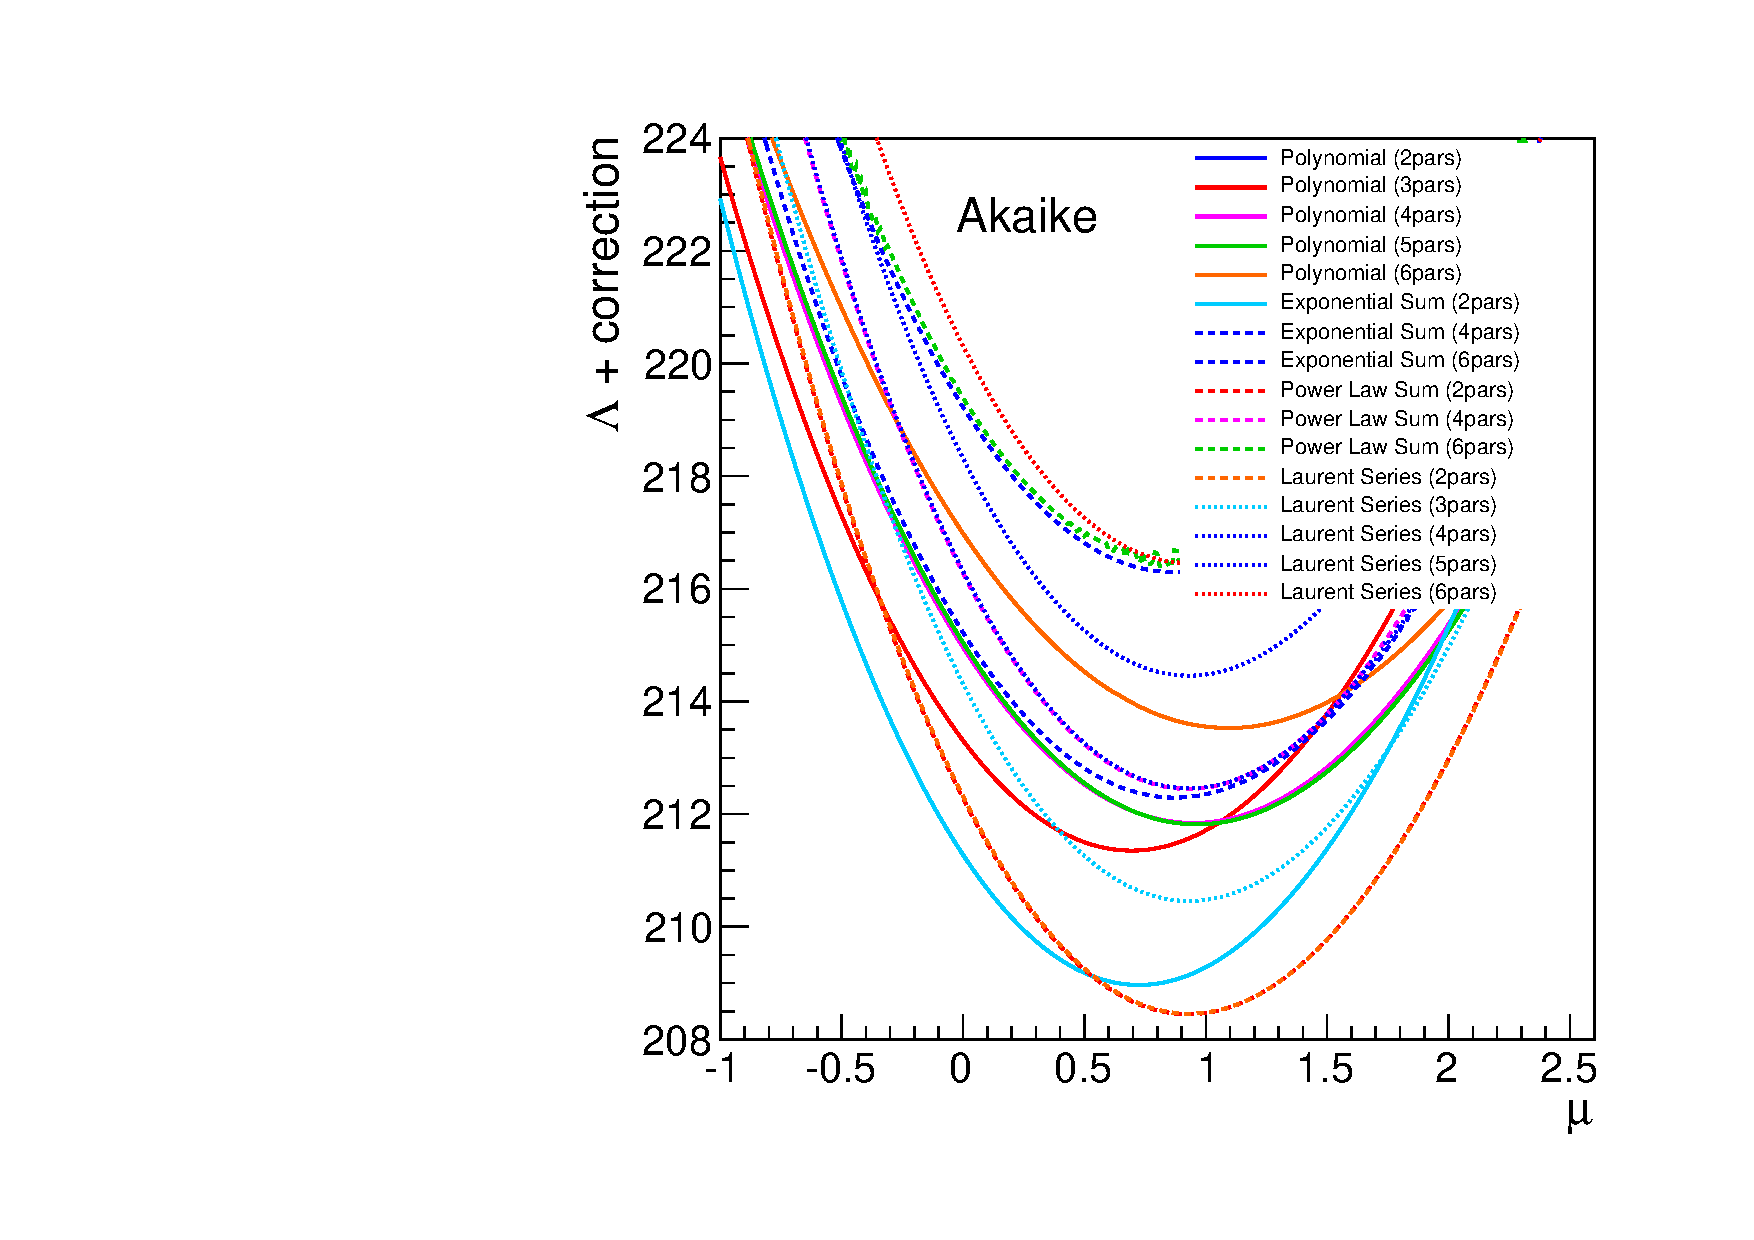
\includegraphics[width=0.46\textwidth]{{correction/ProfilesAllOrders2.0}.pdf}
 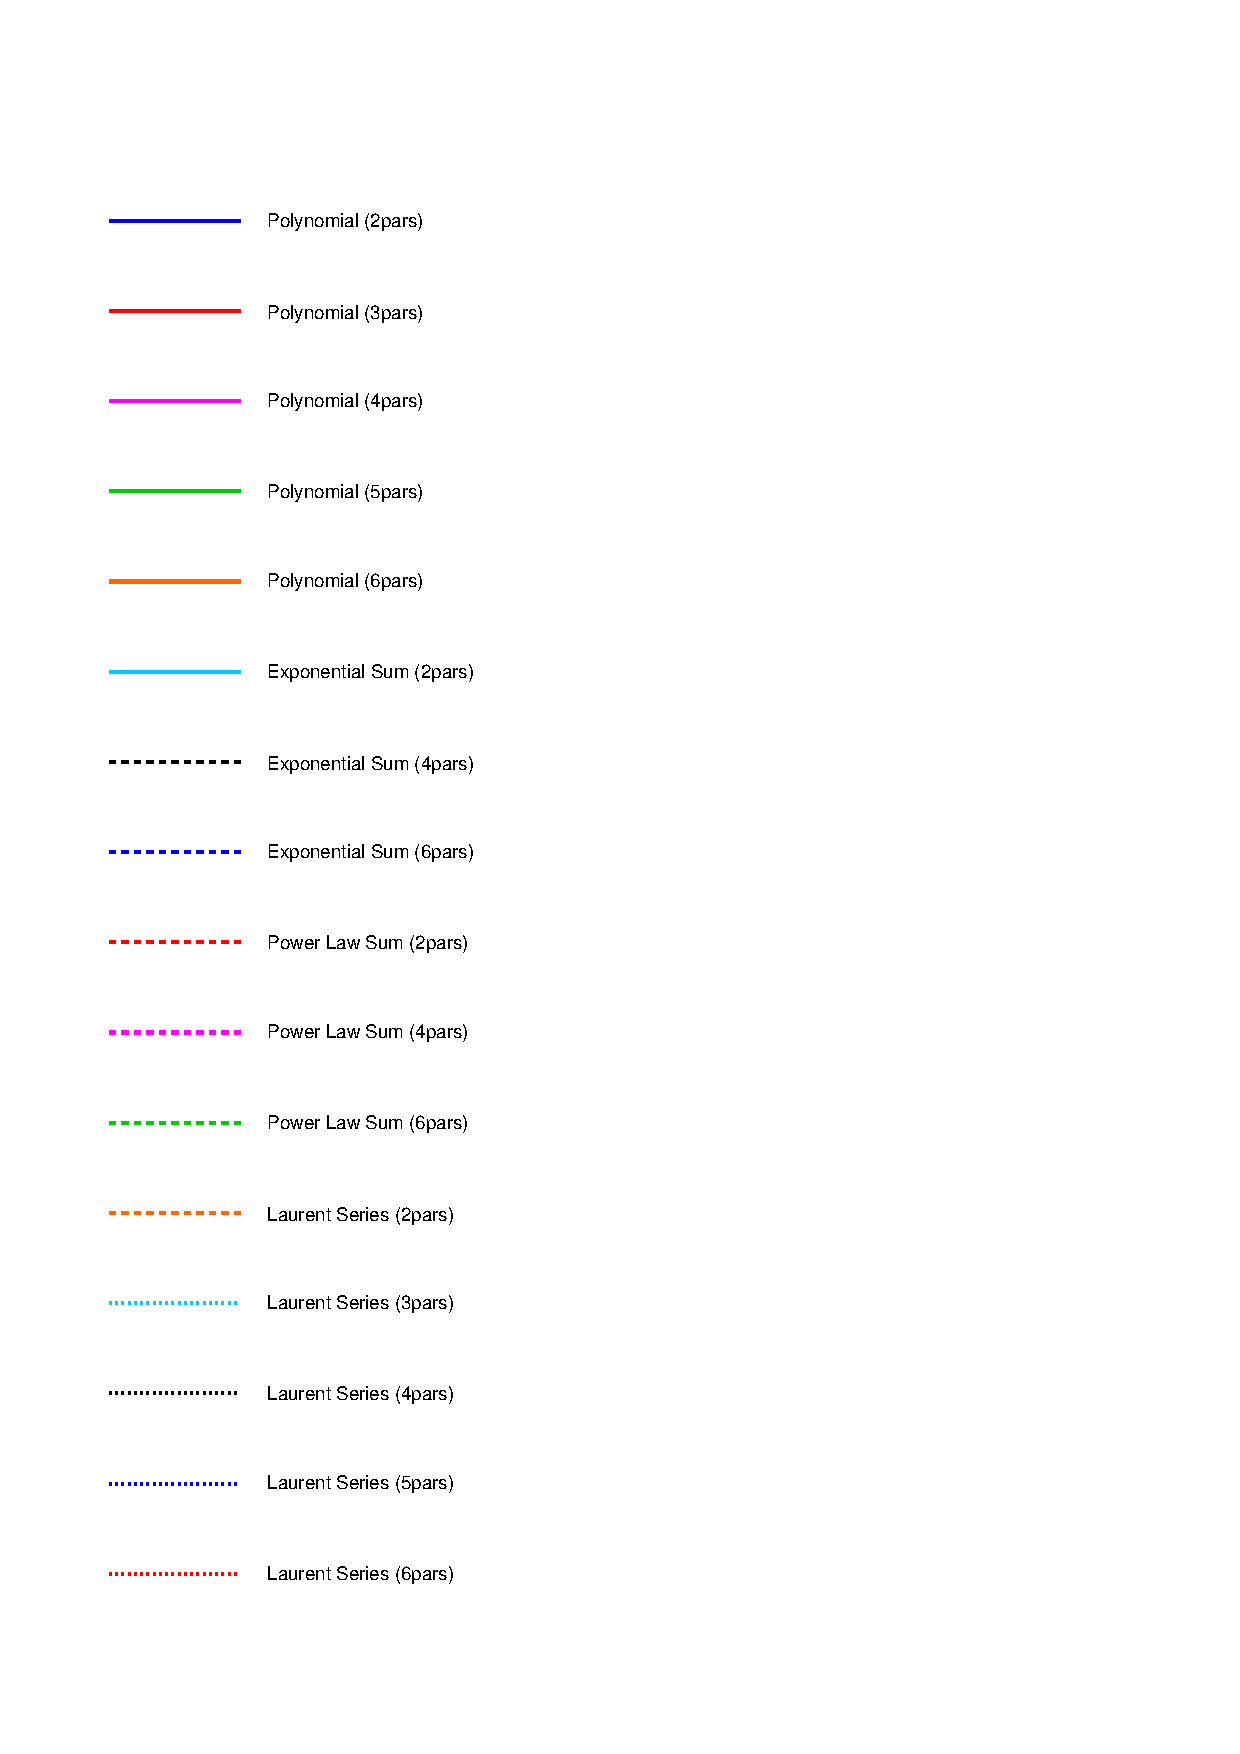
\includegraphics[width=0.46\textwidth]{{correction/AllFunctionsLegend}.pdf}
\label{fig:correction:profiles-akaike:a}
}
\subfigure[]{
 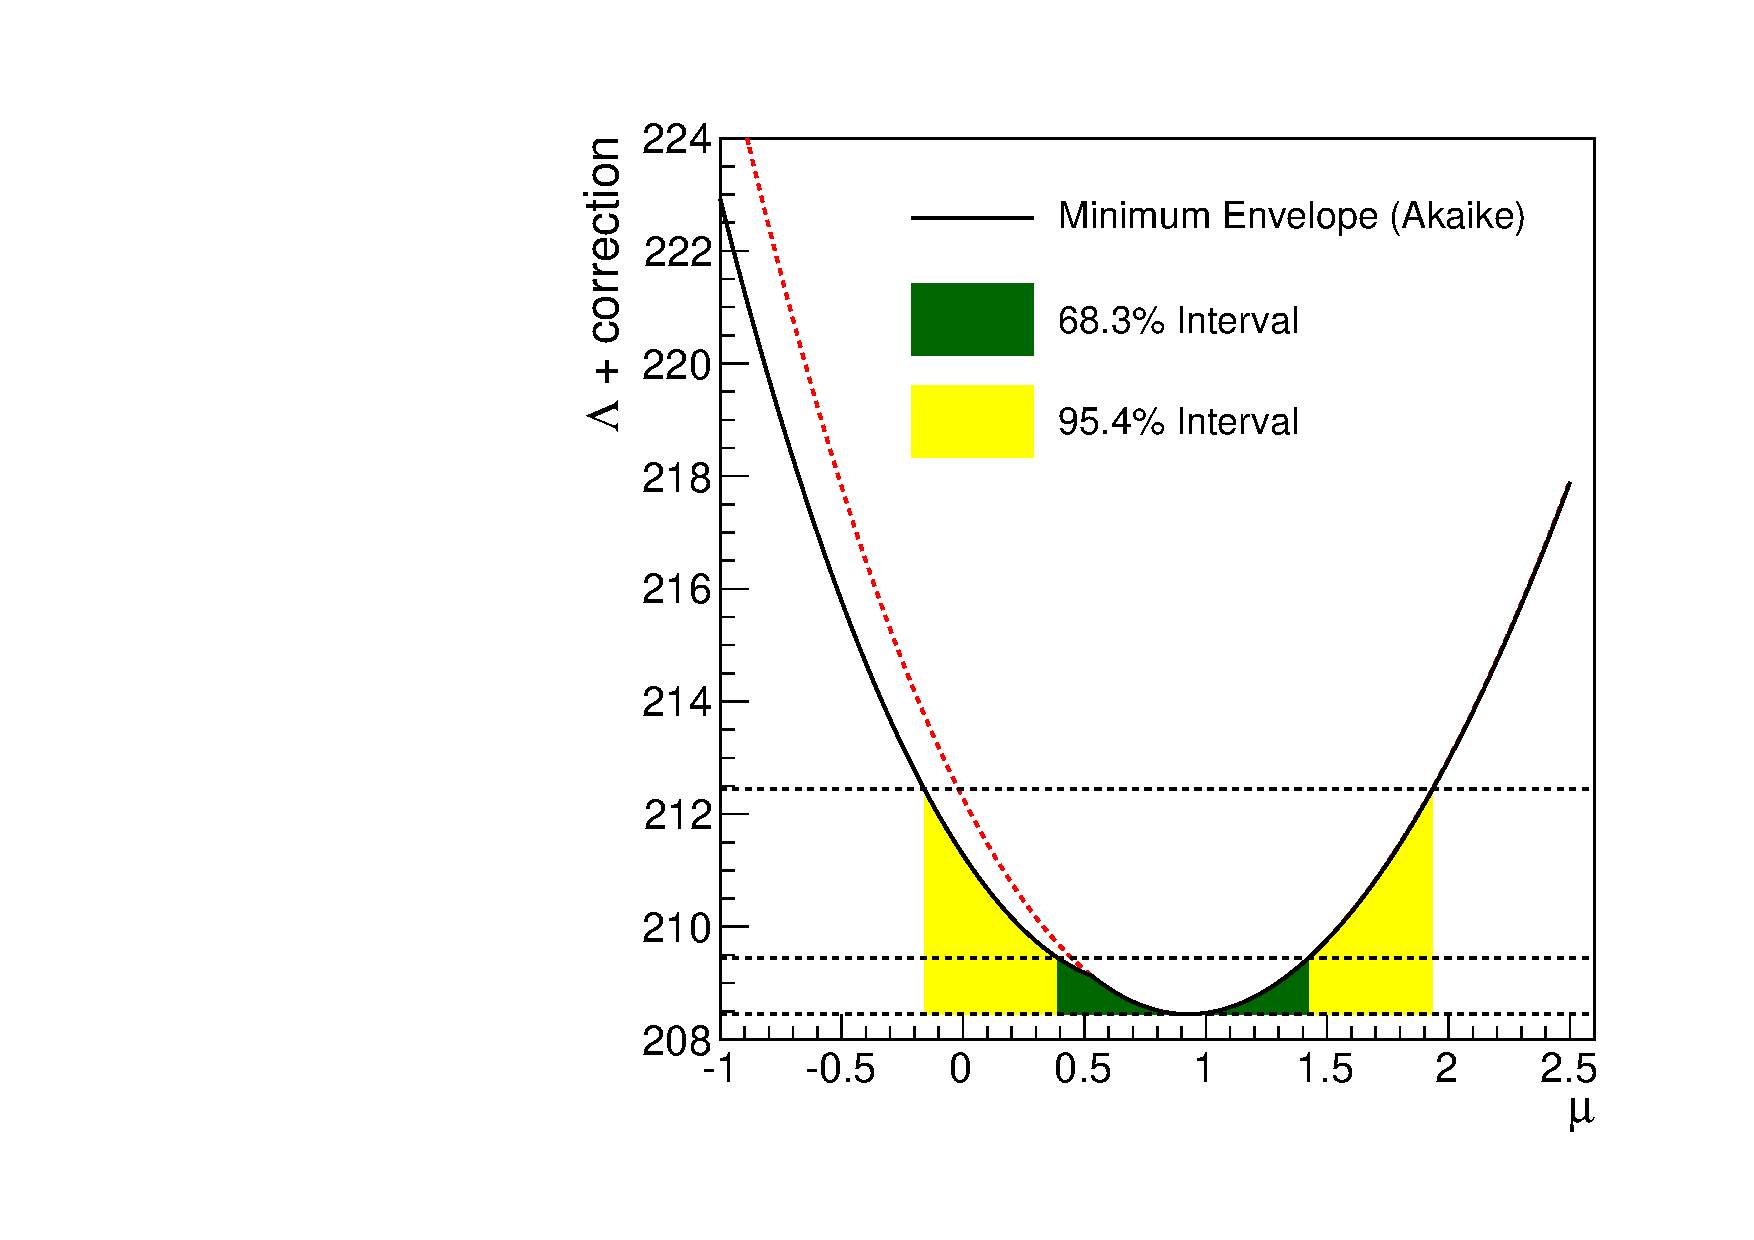
\includegraphics[width=0.46\textwidth]{{correction/EnvelopeAllOrders2.0}.pdf}
\label{fig:correction:profiles-akaike:b}
}
\caption{(a) Profiled \nll curves for all of the functions considered. The \nll value for each profile curve has been corrected using the Akaike correction of 2 per background parameter. The labels indicate the function and the value of $N_{\rm par}$. (b) Minimum envelope of the functions after applying a correction of 2 per background parameter to each \nll curve. The \nll scan when only considering the best fit function is shown in red.}
\label{fig:correction:profiles-akaike}
\end{figure}


In contrast, the case with no correction to \nll, shown in
figure~\ref{fig:correction:profiles-no}, shows that the highest order polynomial
function used, with $N_{\rm par}=6$, defines the envelope across the whole
range of $\mu$. This domination of the functions with the highest numbers of
parameters is exactly what the penalty correction to \nll is attempting to
avoid. Finally, figure~\ref{fig:correction:profiles-akaike},
corresponding to the Akaike correction, shows that all functions with more
than the minimum of two parameters get a large penalty and so do not
contribute to the envelope. This hints that this correction may be too severe.

The three corrections shown can be
considered to be examples of a continuous spectrum of corrections which can
be written as
\begin{displaymath}
\Lambda_{\mathrm{corr}} = \textrm{\nll} + cN_{\rm par},
\end{displaymath}
where $c=0$, 1 or 2 in the cases shown. Other values of $c$ are clearly
also possible.
Figure~\ref{fig:correction:correction} shows the
68.3\% and 95.4\% intervals which would be derived from the envelopes
for these and
some other values of $c$, as well as for the exact p-value correction.
It is seen that the best fit value and intervals change for $c<0.5$ but
for larger values of $c$ they are quite stable. Hence, the result which would
be derived from this method is effectively insensitive to the exact correction
used, as long as $c \gtrsim 1$.
%
\begin{figure}[htp]
\centering
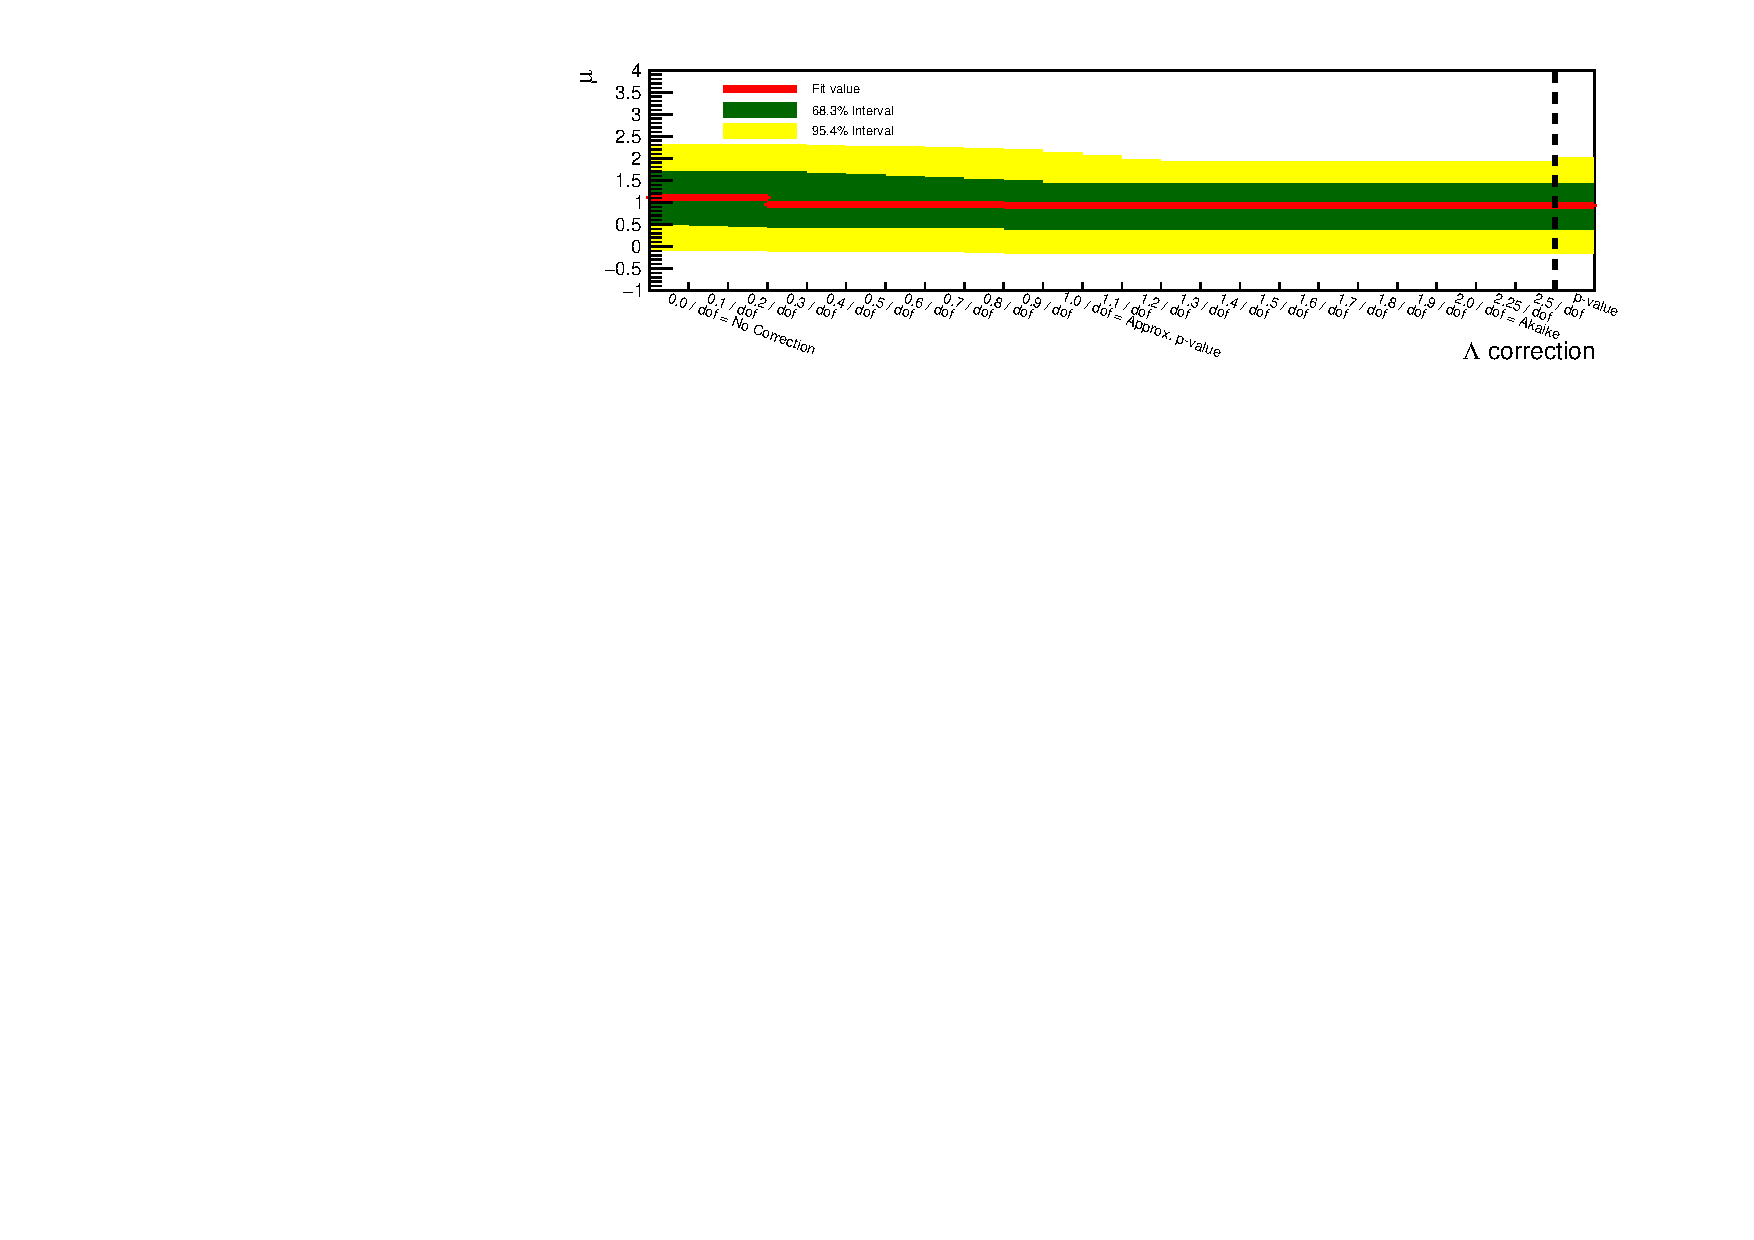
\includegraphics[angle=90,width=0.38\textwidth]{correction/correction.pdf}
\caption{The best fit value of the signal strength, $\mu$, and its uncertainty when fitted to the dataset as a function of the correction applied per background parameter.}
\label{fig:correction:correction}
\end{figure}


%RELATION TO BIAS WHEN USING FUNCTION A TO FIT FUNCTION B? ASIMOV?

%\subsection{Toy generation}
%\label{sec:correction:toys}

%EXTRA COMPLICATION WITH BAYESIAN AND FREQUENTIST MIXTURES OF NORMALISATION

\subsection{Bias and coverage dependence on correction}
\label{sec:correction:bias}

In a similar way to Section~\ref{sec:functions:coverage}, toy datasets
were generated using various individual functions and also the best fit
functions for each $\mu$ value.

Figure~\ref{fig:correction:chisq} shows examples of
the distribution of the difference
in \nll between the true and best fit values of $\mu$. These are shown for the
three correction methods considered. In each case, the function used to generate
the toy datasets was the one giving the best fit as determined from the 
envelopes in figures~\ref{fig:correction:profiles-no}, 
\ref{fig:correction:profiles-pval} and
\ref{fig:correction:profiles-akaike}.
Similarly to figure~\ref{fig:functions:chisq}, these indicate that the
change in \nll is similar to the expected $\chi^2$ distribution and so
is a reasonable basis on which to estimate the uncertainty using an
asymptotic approximation.
%
\begin{figure}[tbp]
\centering
 \subfigure[]{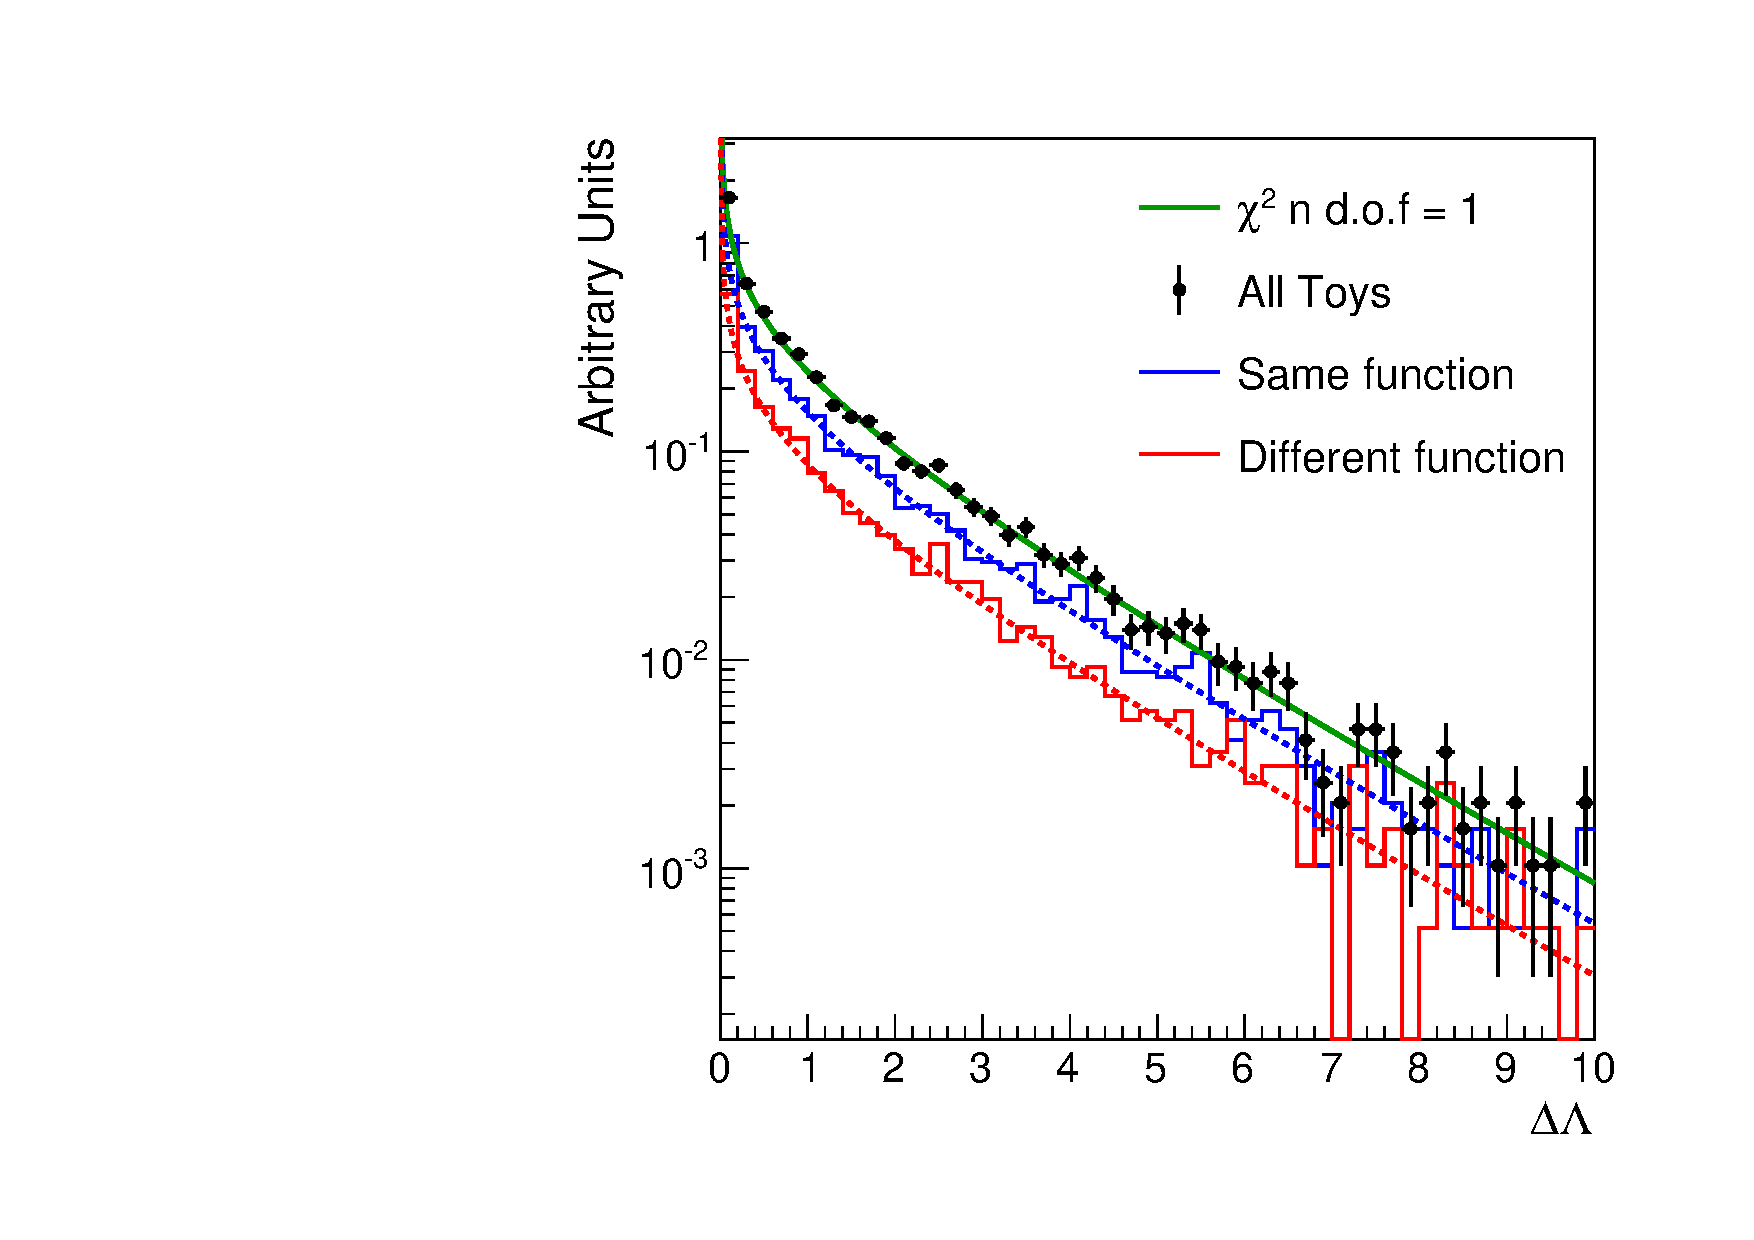
\includegraphics[width=0.32\textwidth]{correction/gen_bern5_mu1_bias_hists_Correcion_0.pdf}
\label{fig:correction:chiSq:a}}
 \subfigure[]{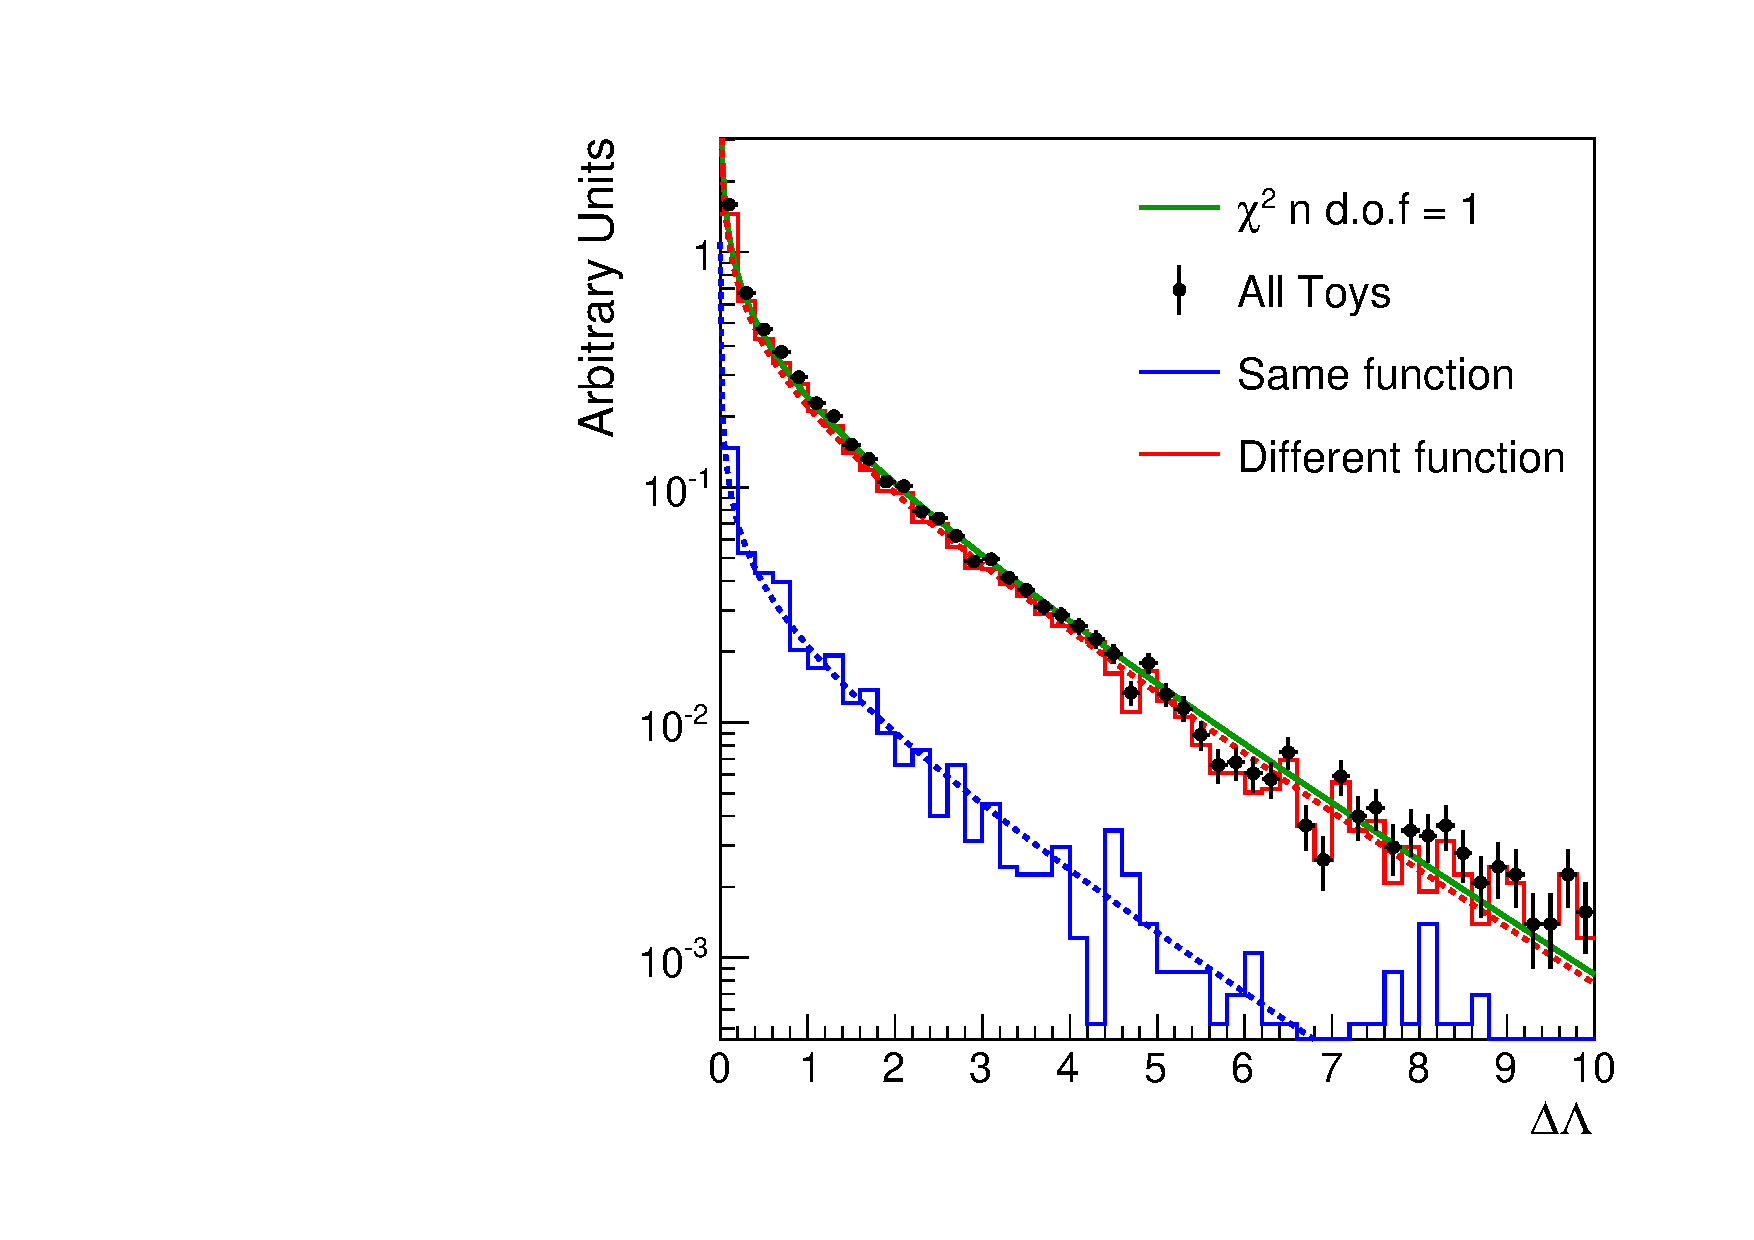
\includegraphics[width=0.32\textwidth]{correction/gen_pow1_mu1_bias_hists_Correcion_1.pdf}
\label{fig:correction:chiSq:b}}
 \subfigure[]{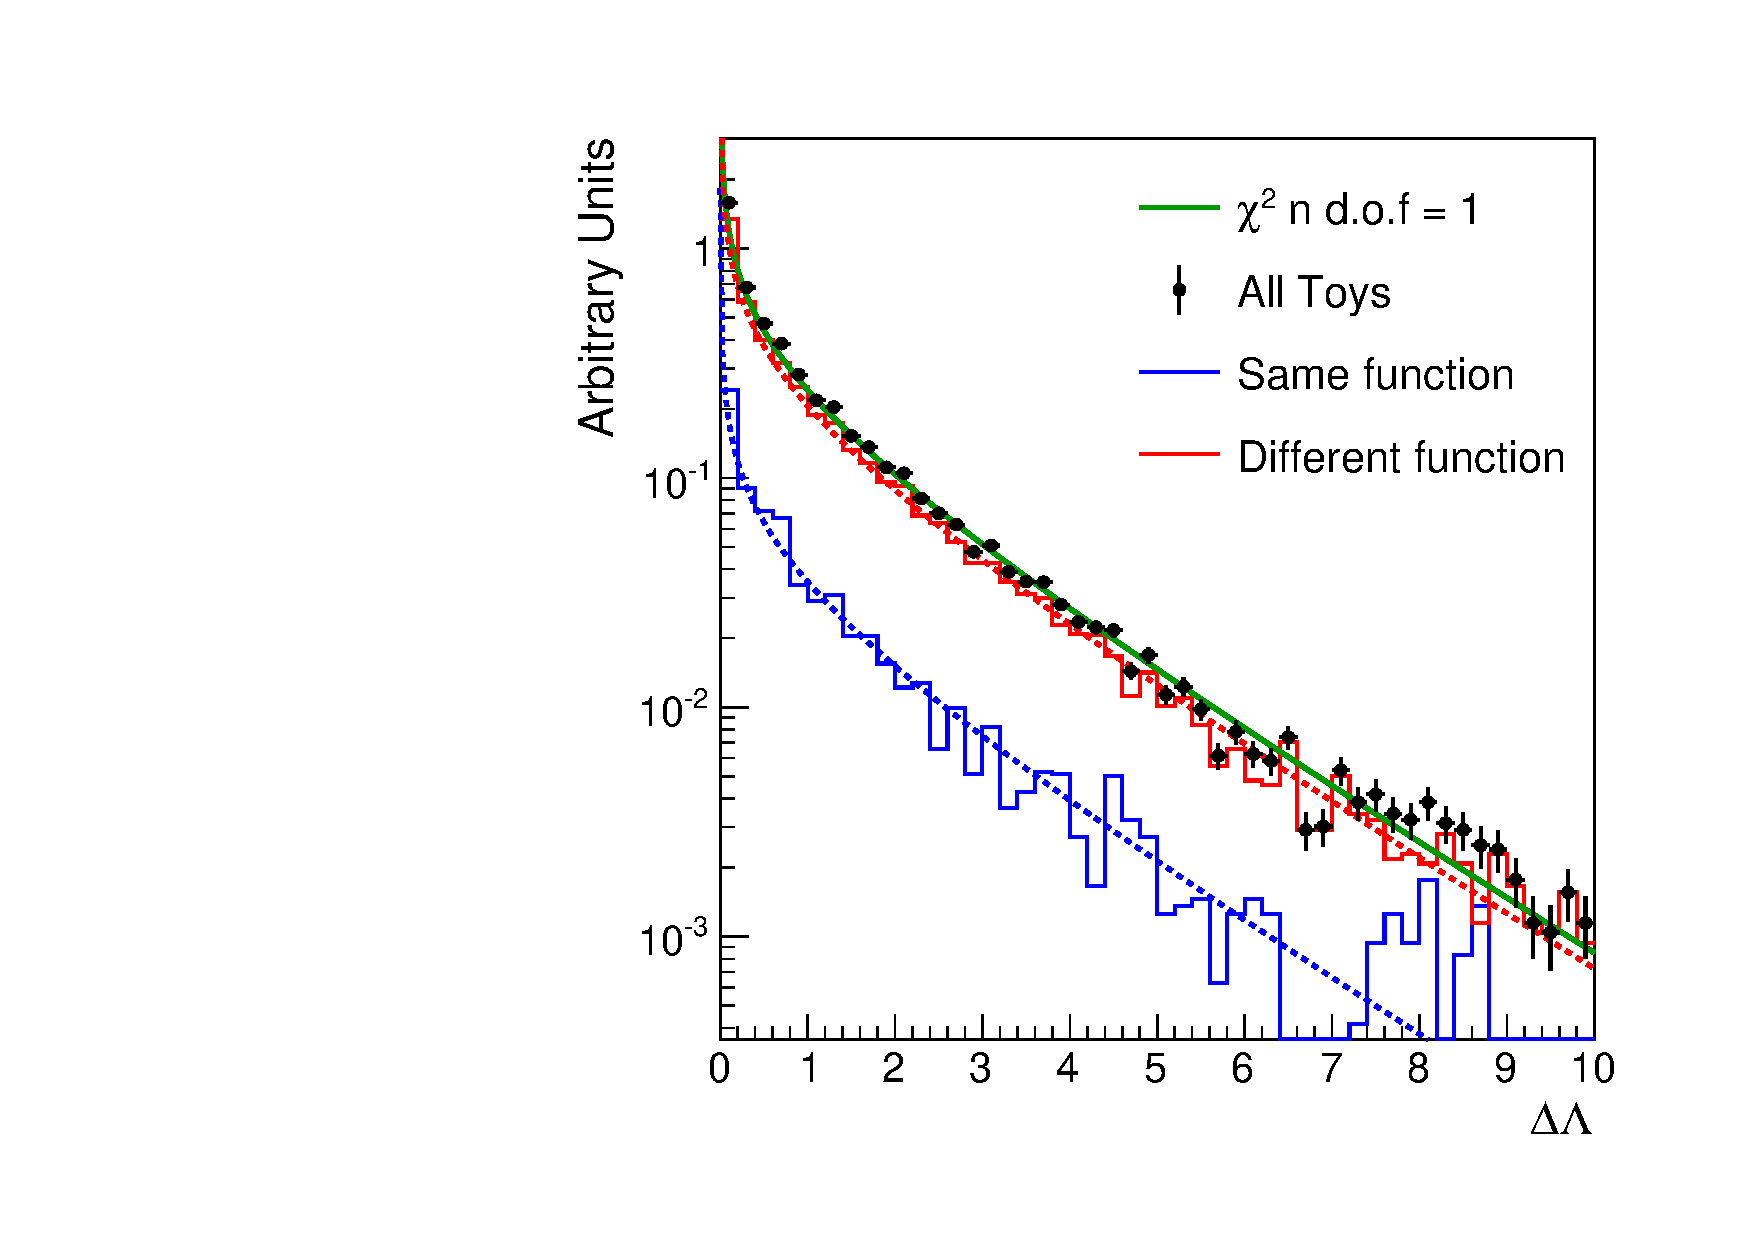
\includegraphics[width=0.32\textwidth]{correction/gen_pow1_mu1_bias_hists_Correcion_2.pdf}
\label{fig:correction:chiSq:c}}
\caption{Distribution of  $\Delta\nll$, the difference
between the \nll value with $\mu$ fixed to its true value and \nll at the best fit value
of $\mu$, (a) with no correction to \nll, (b) with the approximate p-value
correction, and (c) with the Akaike correction.
The black data points are from the toy dataset fits and the green function
shows the expected $\chi^2$ distribution for one degree of freedom.
The blue and red histograms show the toy values separated into
cases where the best fit uses the same or different functions, respectively, compared with the function used to generate the toys.}
\label{fig:correction:chisq}
\end{figure}


Figure~\ref{fig:correction:allorderbias} shows the average pull vs $\mu$
for each choice of generating function, with the envelope based on the
three correction methods considered, i.e.~approximate p-value, p-value
and Akaike.
The generating functions chosen were those
which gave the lowest corrected \nll values in
figure~\ref{fig:correction:profiles-pval}.
Some obvious biases are seen, in particular for the cases when
generating with polynomials of five or six parameters. It seems that in these
cases, which are among the functions with the highest numbers of parameters,
the generated data are too complex to be described well by the lower order
functions. The choice of the Akaike correction makes the bias worse, as it
tends to emphasise the contribution of lower order functions to the envelope.
%This effect could be reduced by working with even higher order functions, but
%these were not found to be needed to describe the original data and so were
%not included.

However,
even with the bias being a significant fraction of the error for some functions,
it is seen that the approximate p-value and p-value corrections give
effectively identical results. It is also found
that the p-value corrections always give less bias than the Akaike correction.
%
\begin{figure}[tbp]
\centering
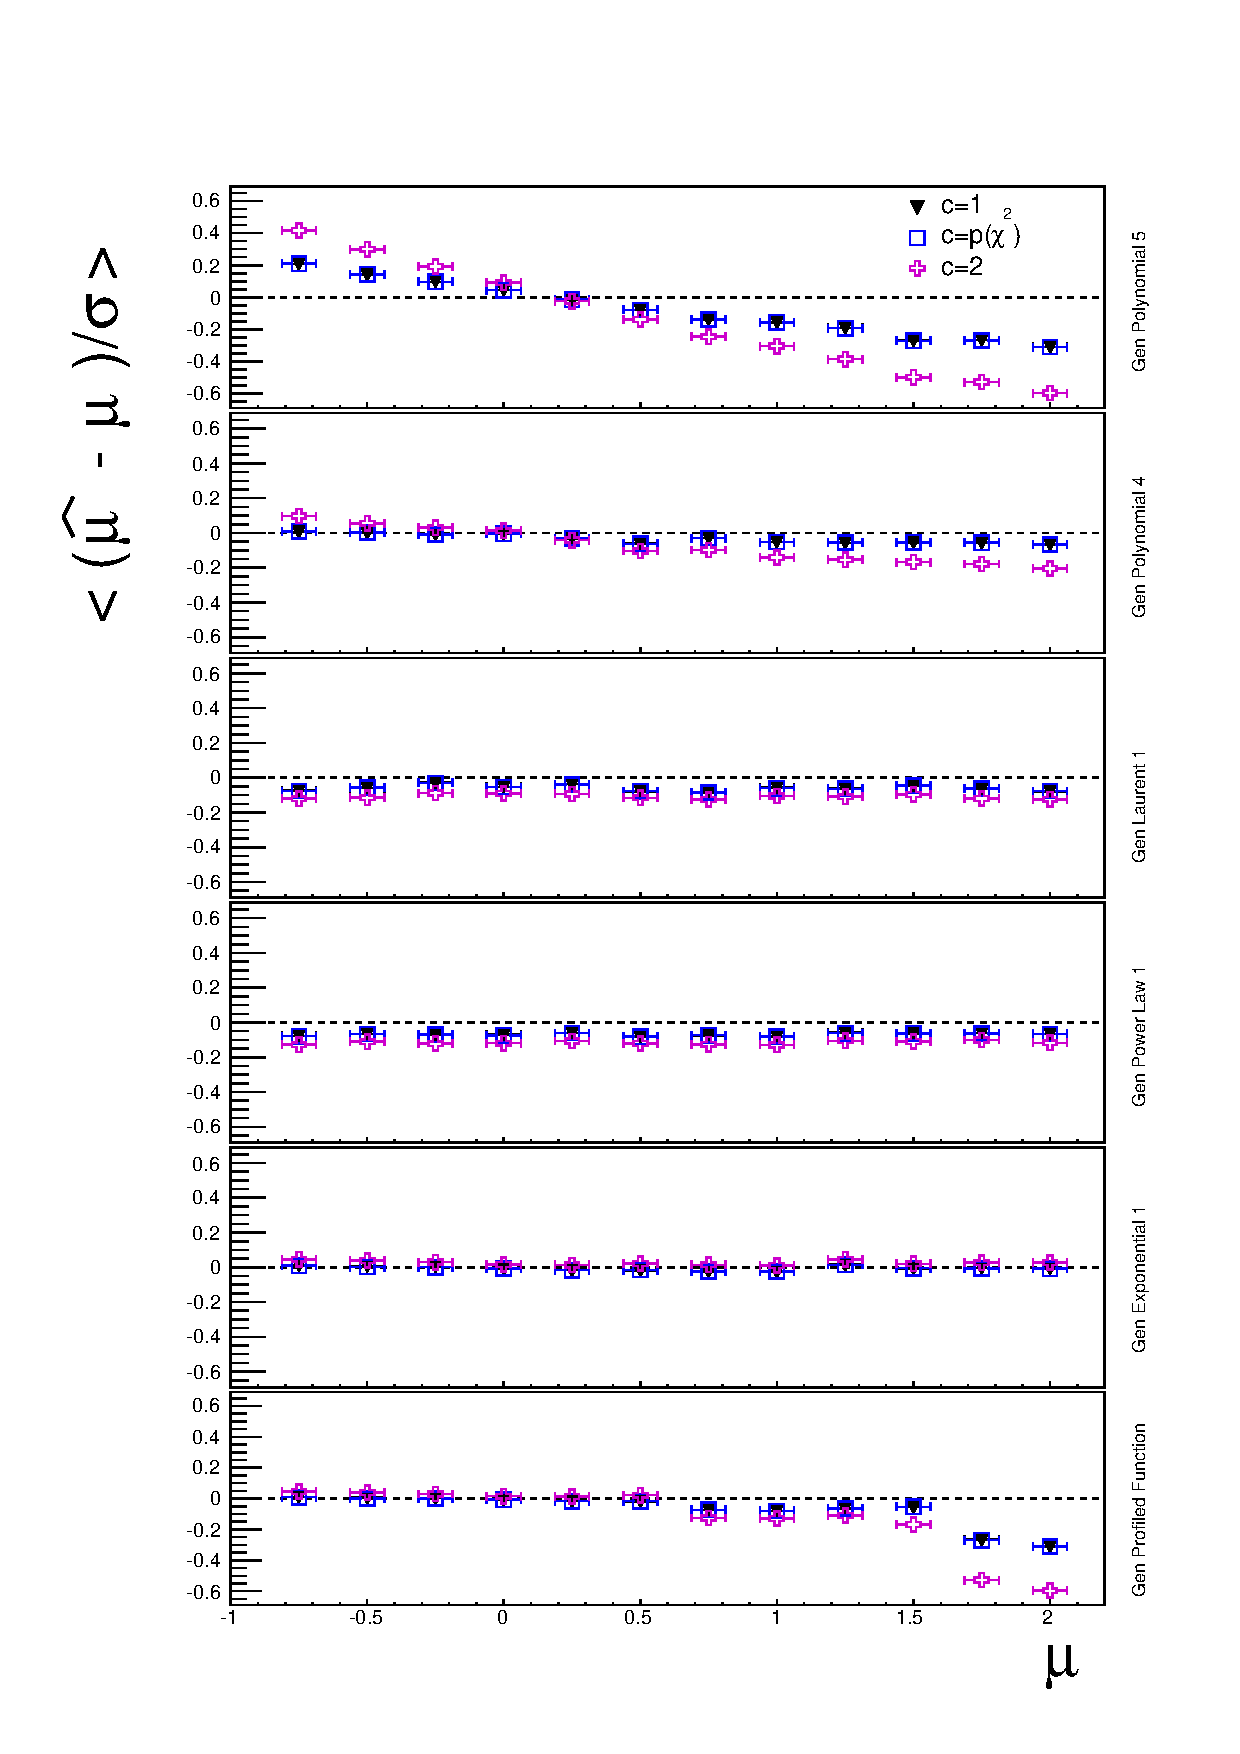
\includegraphics[width=0.8\textwidth]{correction/AllOrderFunctions_call.pdf}
\caption{Average pull when fitting using the envelope as a function of $\mu$
used to generate the signal when correcting
with the different \nll correction schemes.
Each panel shows the bias when using
a different background function for toy generation, with the functions
used being: polynomial with $N_{\rm par}=6$ (a),
polynomial with $N_{\rm par}=5$ (b), Laurent with $N_{\rm par}=2$ (c),
power law with $N_{\rm par}=2$ (d), and exponential with $N_{\rm par}=2$ (e).
Panel (f) shows the result when the best-fit function at each
value of $\mu$ is used to generate toys.
%For each plot, the results for the three correction methods are shown,
%namely the approximate p-value (``$c=1$''), p-value (``$c=p(\chi^2)$'')
%and Akaike (``$c=2$'').
}
\label{fig:correction:allorderbias}
\end{figure}

Similarly, figure~\ref{fig:correction:allordercoverage} shows the fraction of
times the envelope fit result was within the various \nll ranges, as used
previously in figure~\ref{fig:functions:firstordercoverage}. Again, the
coverage is reasonably good for all cases. As for the bias, the two
p-value corrections are very similar and always give better coverage than the
Akaike correction.
%
\begin{figure}[tbp]
\centering
\subfigure[]{
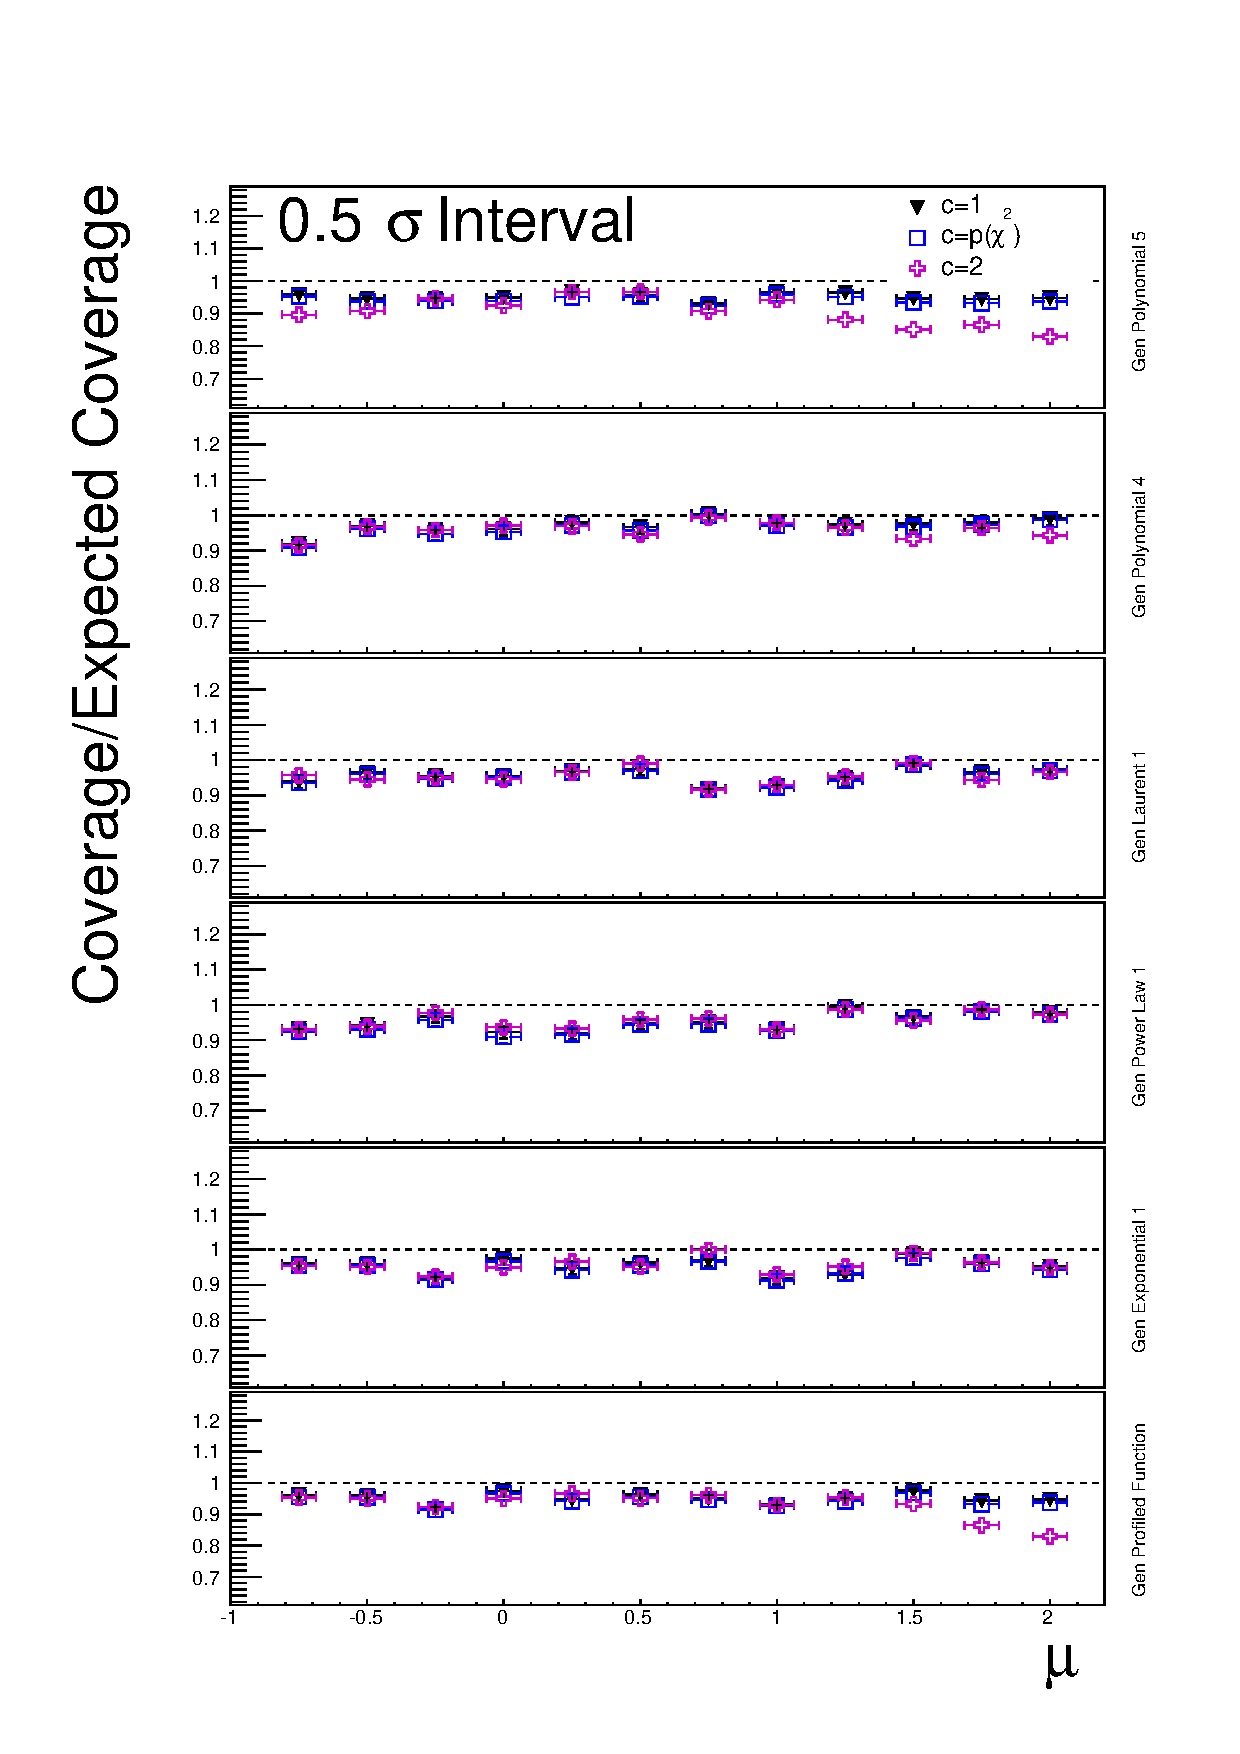
\includegraphics[width=0.40\textwidth]{{correction/AllOrderFunctions_Coverage_0.5_call}.pdf}
\label{fig:correction:allorderecoverage:a}
}
\subfigure[]{
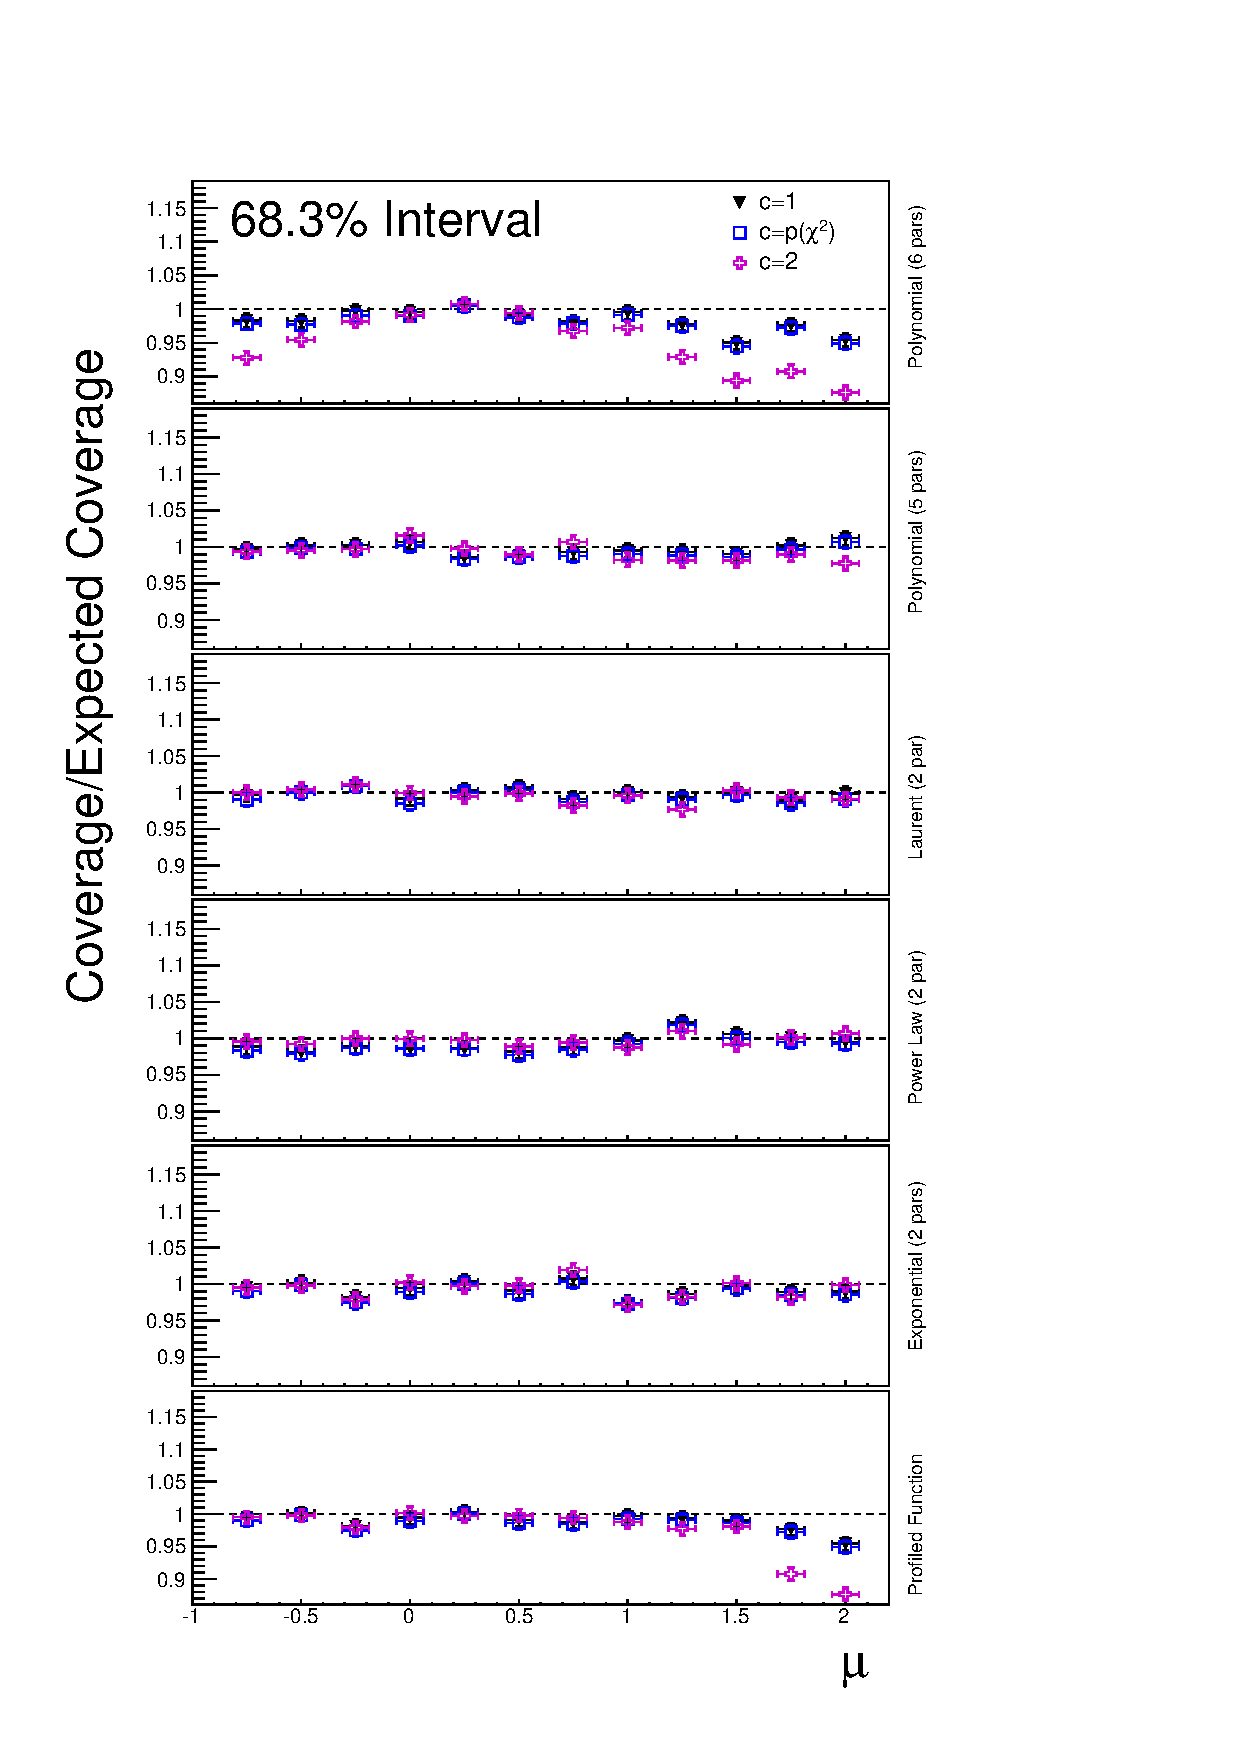
\includegraphics[width=0.40\textwidth]{{correction/AllOrderFunctions_Coverage_1._call}.pdf}
\label{fig:correction:allorderecoverage:b}
}\\
\subfigure[]{
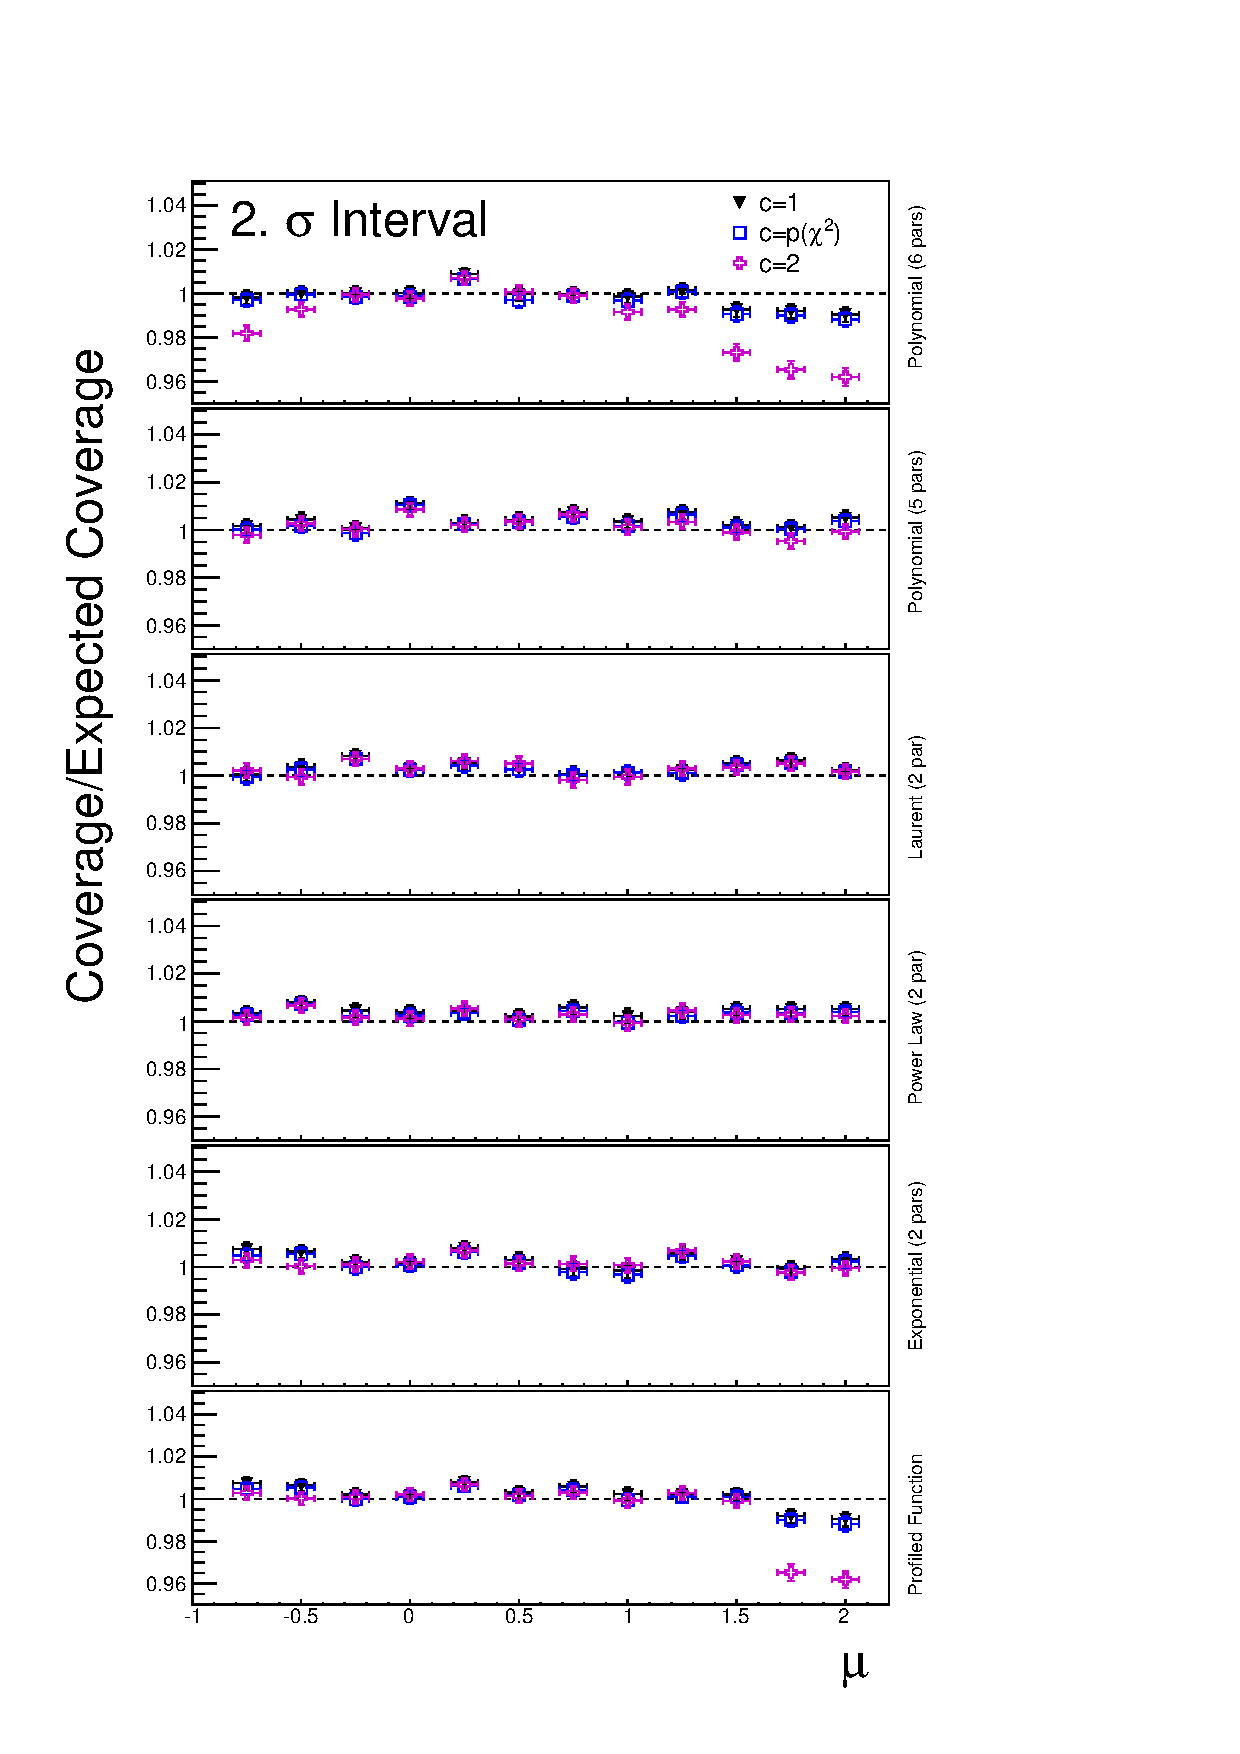
\includegraphics[width=0.40\textwidth]{{correction/AllOrderFunctions_Coverage_2._call}.pdf}
\label{fig:correction:allorderecoverage:c}
}
\subfigure[]{
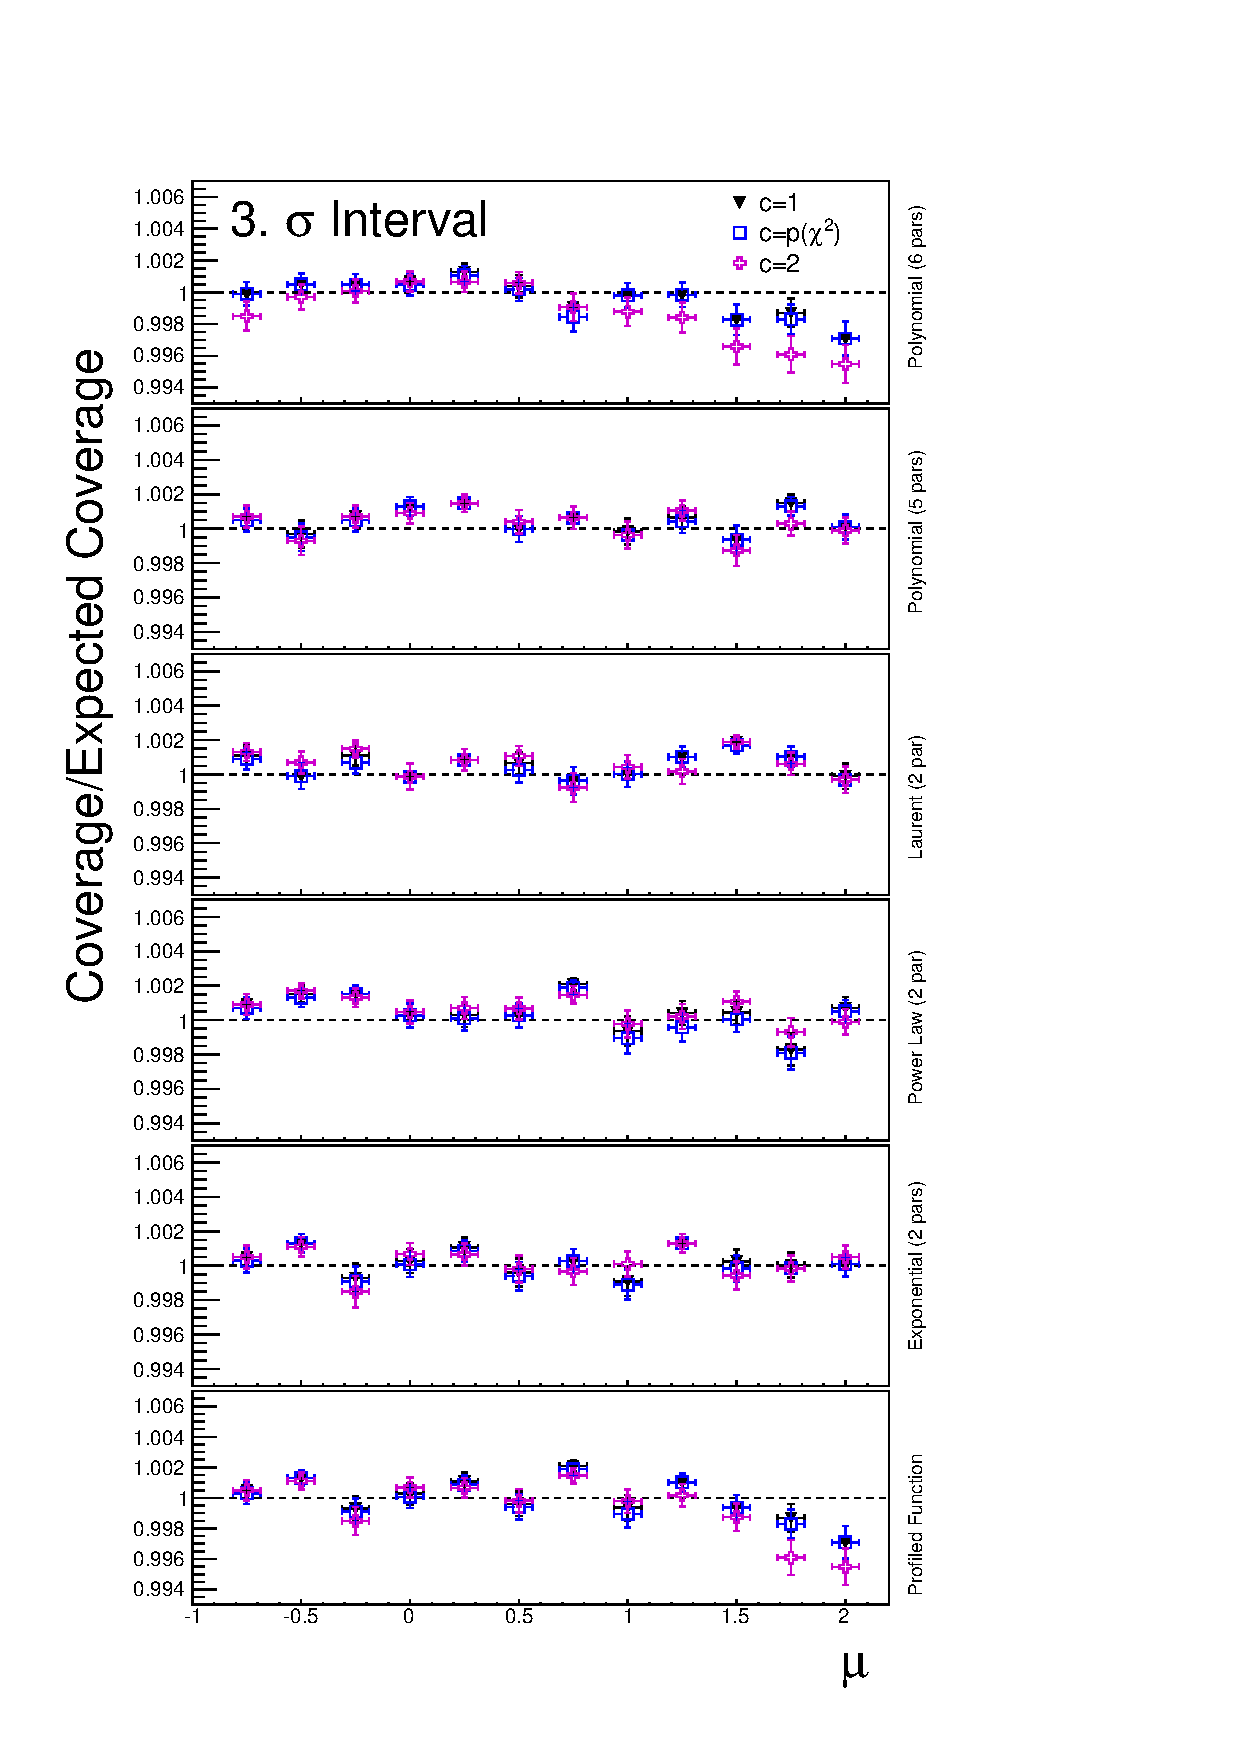
\includegraphics[width=0.40\textwidth]{{correction/AllOrderFunctions_Coverage_3._call}.pdf}
\label{fig:correction:allorderecoverage:d}
}
\caption{
Measure of the fraction of the toys which do not contain the generated
$\mu$ in various specified $\Lambda$ intervals, converted
into the two-sided score $|Z|$,
when correcting
with the different \nll correction schemes.
The intervals are
$\Delta\Lambda$ of 0.25 (a), 1.0 (b), 4.0 (c) and 9.0 (d).
The results when generating with different functions and generating using the
profiled function for each value of $\mu$ are shown in the different panels.
The functions
used are (from the top panel in each case): polynomial with $N_{\rm par}=6$,
polynomial with $N_{\rm par}=5$, Laurent with $N_{\rm par}=2$,
power law with $N_{\rm par}=2$, and exponential with $N_{\rm par}=2$.
The lowest panel in each case shows the result when the best-fit function at each
value of $\mu$ is used to generate toys.
%For each plot, the results for the three correction methods are shown,
%namely the approximate p-value (``$c=1$''), p-value (``$c=p(\chi^2)$'')
%and Akaike (``$c=2$'').
}
\label{fig:correction:allordercoverage}
\end{figure}

Hence, overall the two p-value correction methods seem to give effectively
identical results and also perform better than the Akaike correction method.
In practical terms, the approximate p-value correction method is easier
to implement than the exact method
and also can be applied to an unbinned fit (where the $\chi^2$
is not approximately given by the \nll value). For these reasons, the approximate
p-value correction was used throughout the CMS Higgs
to two photon analysis~\cite{ref:introduction:legacy}.

Figure~\ref{fig:correction:compareerrors} shows the distribution of the 68.3\%
 uncertainty on $\mu$
when considering the full set of functions using the three different correction schemes compared
with considering a single first order function. The uncertainty ($\sigma_{\mu}$)
is defined as half of the 68.3\% interval on $\mu$.
The distributions are obtained from fitting
toy datasets generated using the first order power law function for the background, with
signal generated assuming $\mu=1$. This quantifies the increase in the error
due to the systematic contribution arising from the uncertainty in the choice of functional form.
The second peak in the distributions observed
when considering the envelope of functions are due to cases in which functions other than the
best fitting function contribute to the 68.3\% interval. As expected, correcting using a higher
penalty reduces the size of this tail since in this case, it is less likely that a higher order
function can contribute.

\begin{figure}[tbp]
\centering
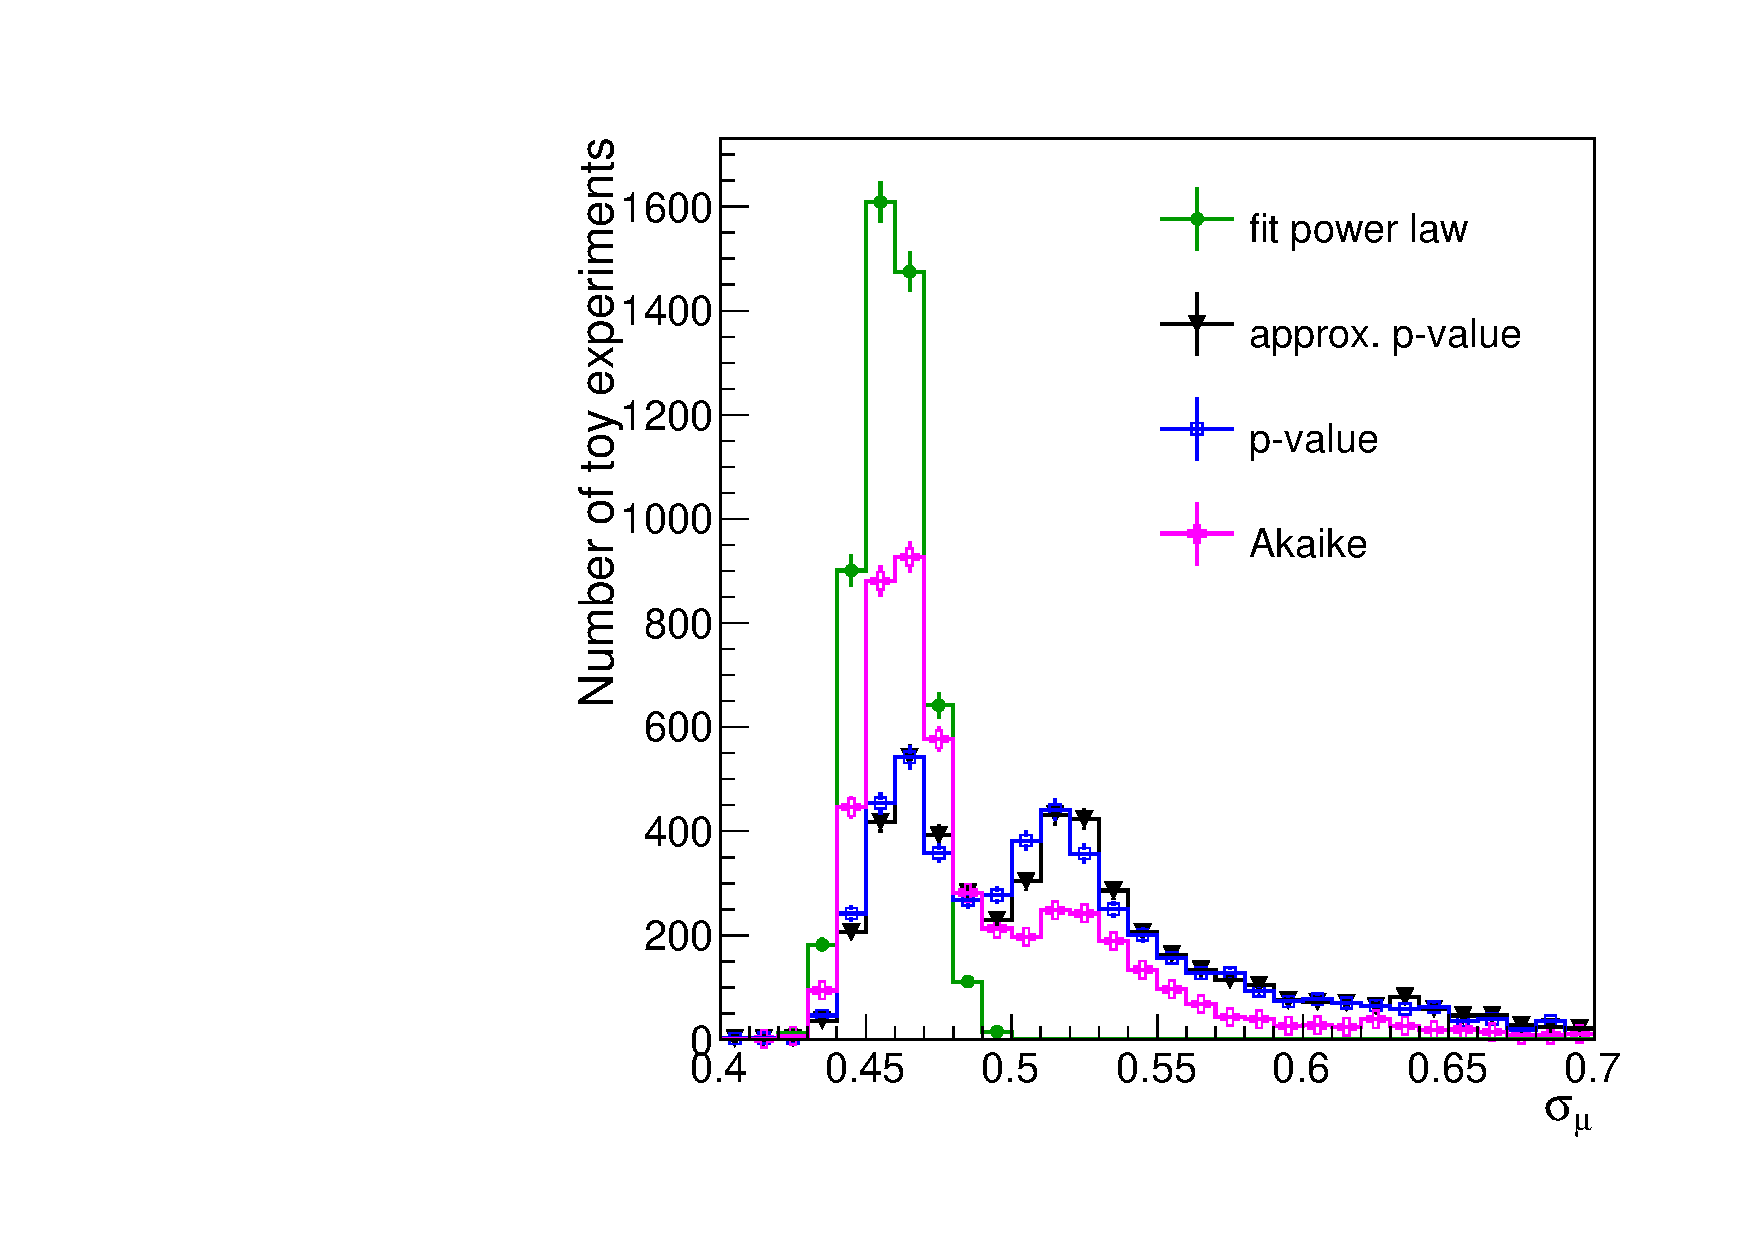
\includegraphics[width=0.45\textwidth]{correction/compare_error_magnitude.pdf}
\caption{Distribution of $\sigma_{\mu}$ in toy datasets
comparing the three correction schemes
when including the full set of functions
with the case when considering only a single power law function
with $N_{\rm par}=2$ for the fit.}
\label{fig:correction:compareerrors}
\end{figure}

\subsection{Comments on the choice of correction}
\label{sec:correction:comments}
 As mentioned at the end of Section~\ref{sec:correction:example},
the correction can be considered to have the form
\begin{displaymath}
\Lambda_{\mathrm{corr}} = \textrm{\nll} + cN_{\rm par},
\end{displaymath}
giving a continuum of possible values of $c$, not just $c=1$ or 2.
Figure~\ref{fig:correction:allordercoverage} indicates that in most cases, the
coverage is effectively independent of the value of $c$. This means that,
within a reasonable range,
the value of $c$ used can be motivated by other considerations. In general,
the choice of a particular value of $c$ to use depends on the application
and the amount of data available.

Figure~\ref{fig:correction:allordererrvscorr} shows the mean of the difference
between the best fit $\mu$ value and the true $\mu$, and also the 68.3\%
statistical uncertainty on $\mu$ from the fit, calculated from the toy
samples discussed above, as a function of $c$,
for generated values of $\mu=0$ and 1. It is seen that the $\mu$ offset
is generally small but increases with the correction value $c$. This is
because lower order functions are favoured for large $c$ and these are not as good at
describing more complicated shapes. Note the largest
offset is found when generating with the six-parameter polynomial, as there
are few other functions being used in this study which have a similar number
of parameters.
Conversely, the
statistical error gets smaller for large $c$ as there tend to be fewer parameters
in the functions that contribute to the envelope.

Clearly there is a trade off between statistical power and systematic bias. Furthermore, the
size of this effect is somewhat hidden by the fact that the highest order functions considered
in this example only go up to six free parameters. If even higher order functions were considered
the statistical uncertainty at low values of $c$ would become unnecessarily large.

In principle, the results of figure~\ref{fig:correction:allordererrvscorr}
could be used to choose an ``optimal'' value of $c$
for a given dataset. Here, optimal means in some way trying to minimise
the overall uncertainty, which arises from some combination of
the bias and the statistical error.
It is clear that such an optimal value will change with the
amount of data as the
statistical errors will become smaller but the offset will stay the same and
hence lower values of $c$ will be favoured for larger data volumes.
However, defining how to optimise the value is somewhat arbitrary. It depends
on whether accurately knowing the true uncertainty on $\mu$ is critically
important. The statistical error will be well known but the bias depends on the
underlying background shape which is by definition not well known. Hence,
how to weigh the relative importance of these two contributions is not uniquely
defined. For example, the offset and statistical error could be added in
quadrature to give an estimate of the overall error. For the case of
figure~\ref{fig:correction:allordererrvscorr}, this has its smallest
value at high $c$. However, for the actual Higgs to two photon analysis, the value of $c=1$
was chosen. This is more conservative, in that it means the known statistical
error will dominate.
%
\begin{figure}[tbp]
\centering
\subfigure[]{
 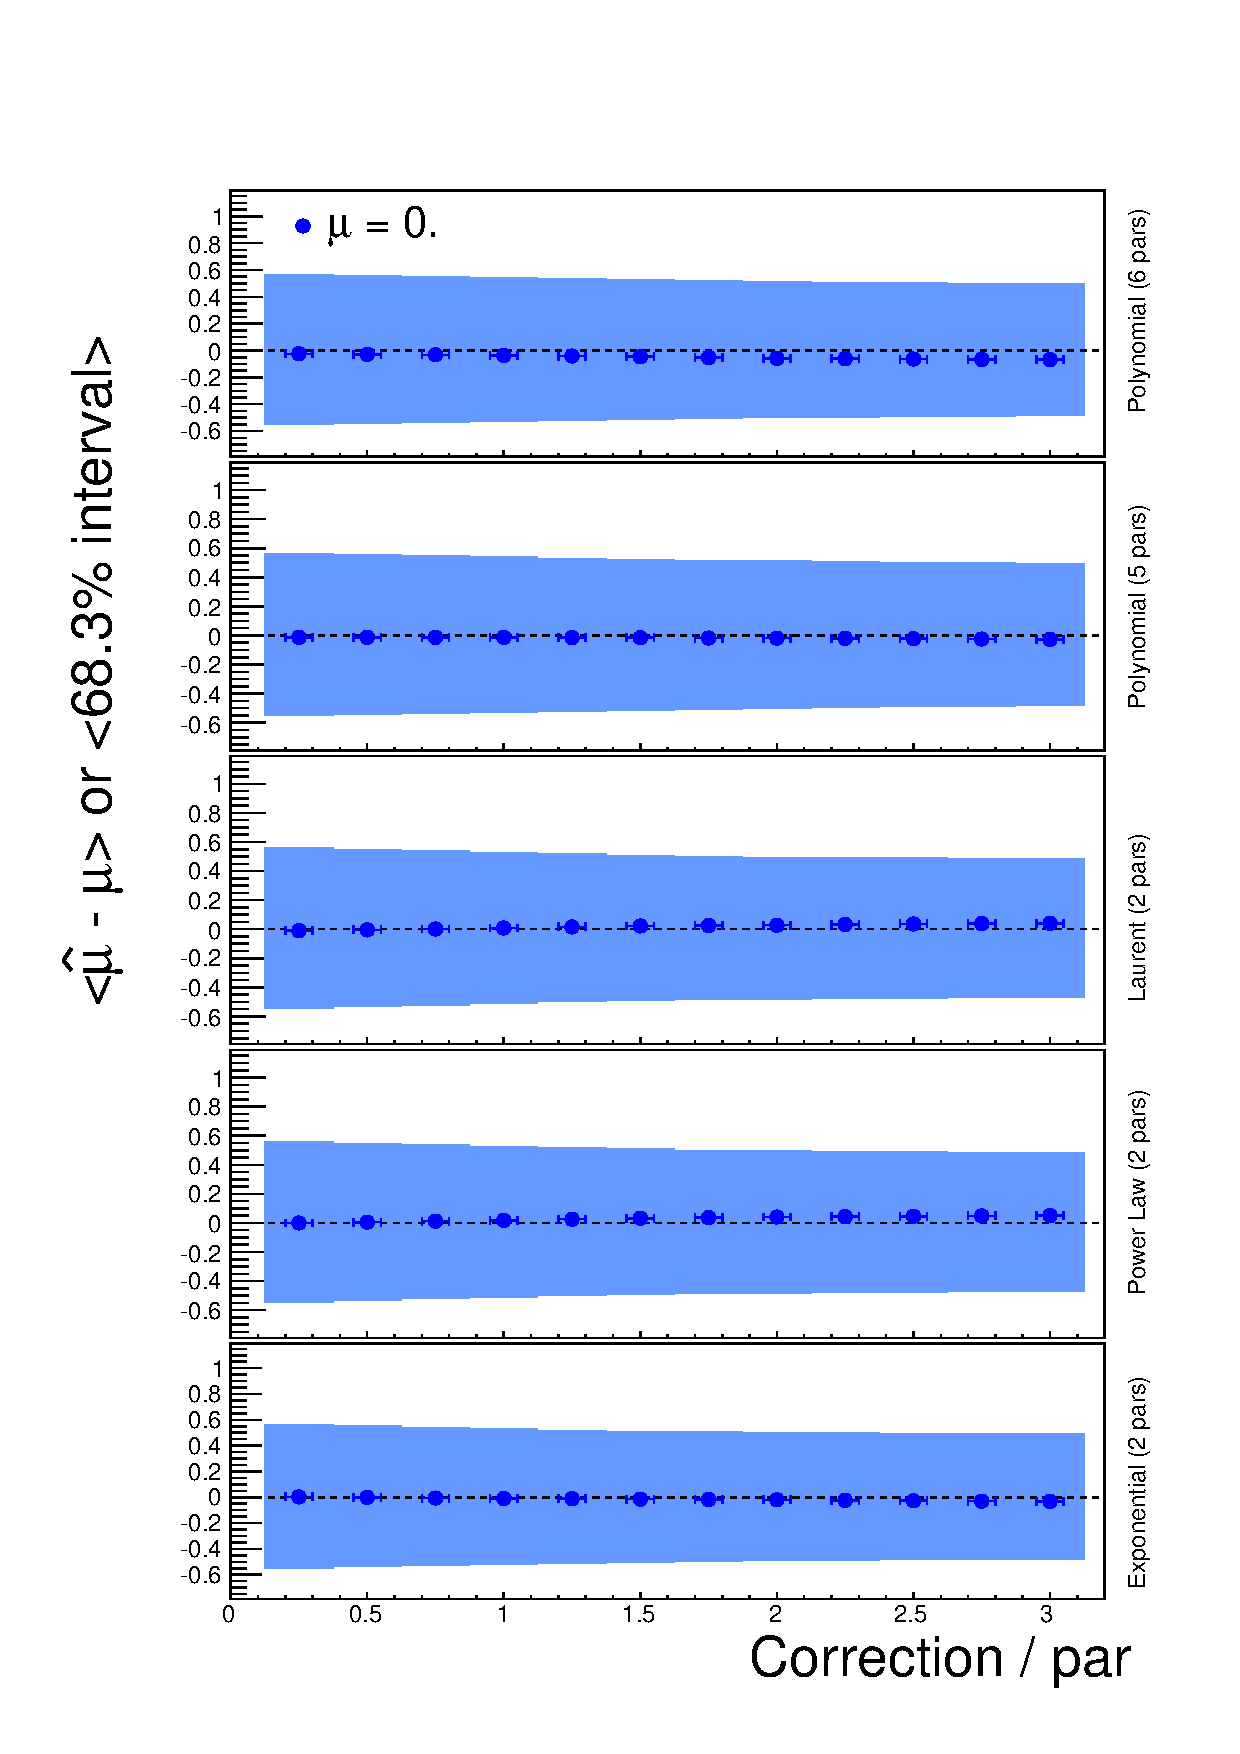
\includegraphics[width=0.46\textwidth]{{correction/AllOrderFunctions_errors_vs_correction_0.}.pdf}
\label{fig:correction:allordererrvscorr-0}
}
\subfigure[]{
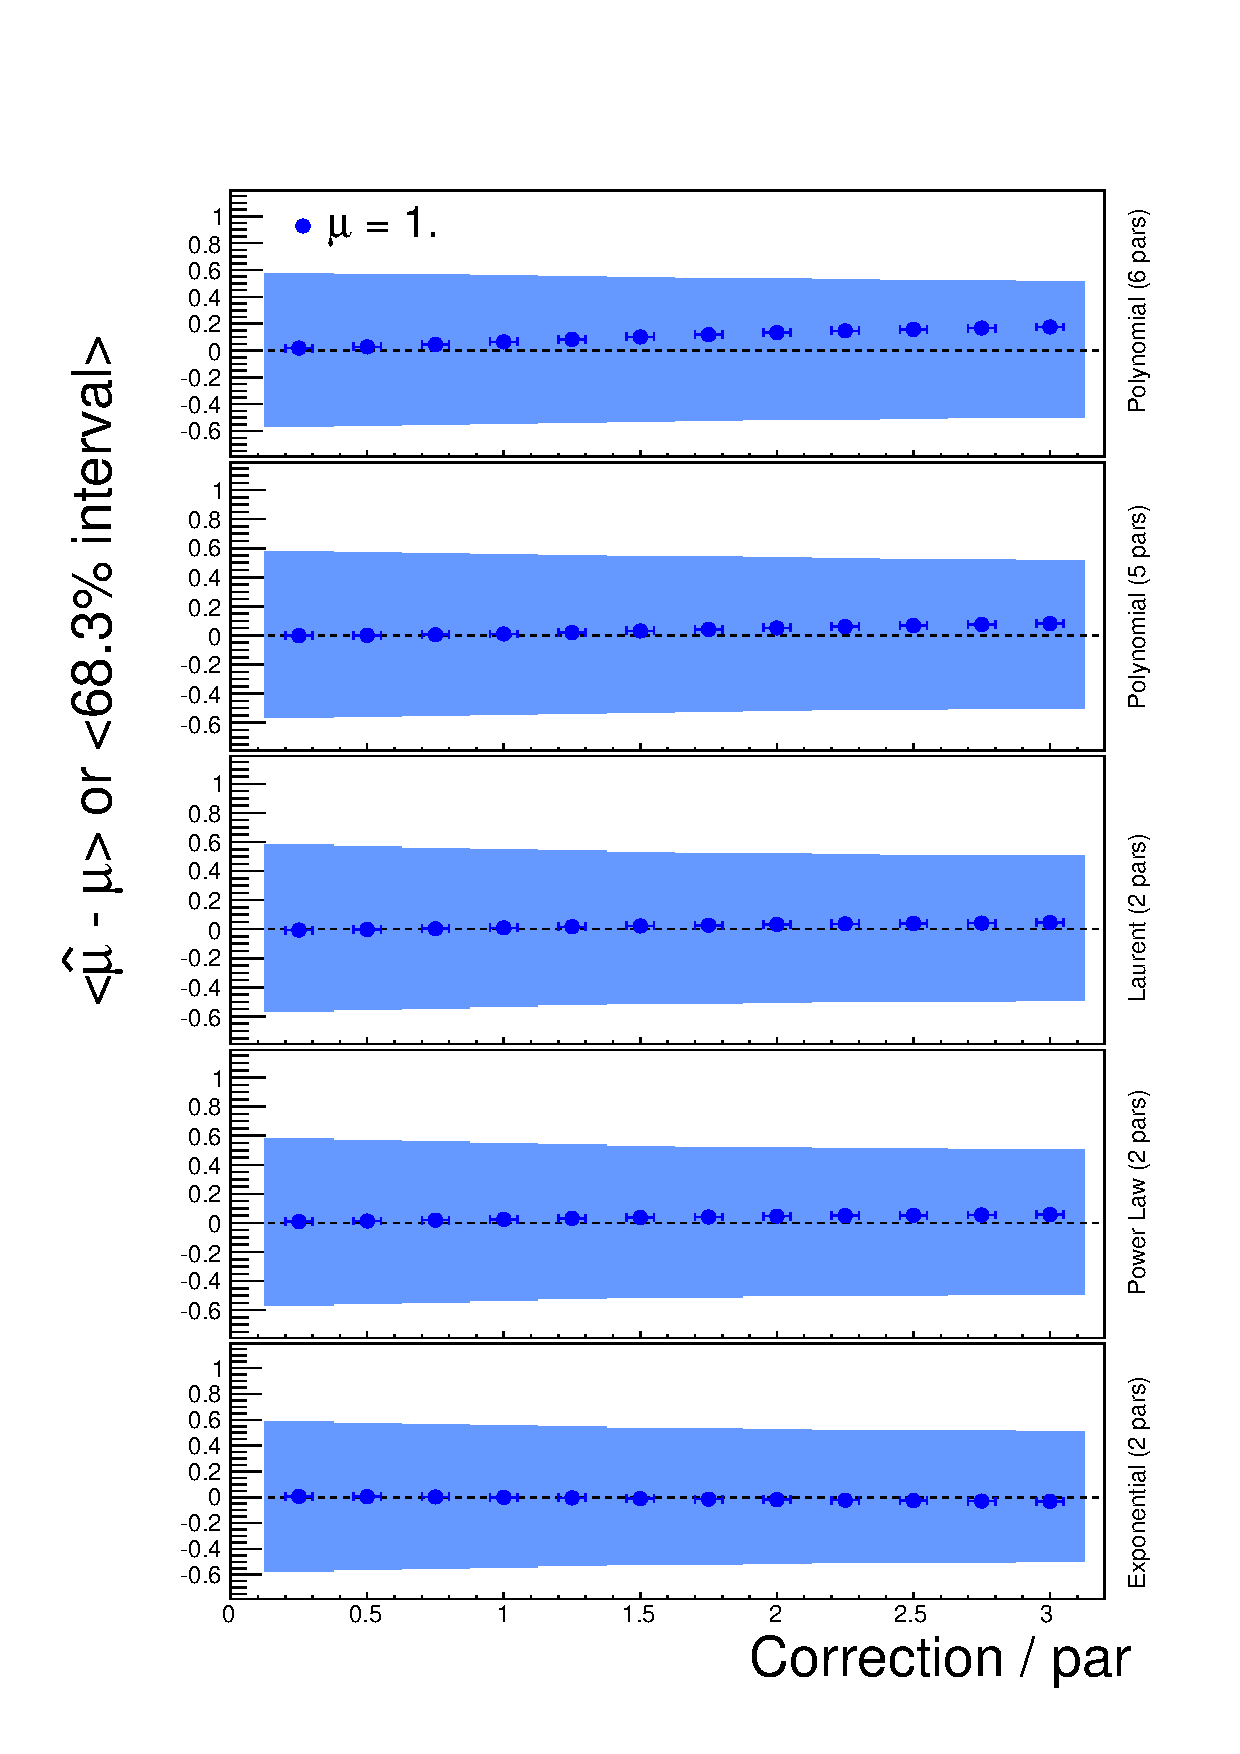
\includegraphics[width=0.46\textwidth]{{correction/AllOrderFunctions_errors_vs_correction_1.}.pdf}
\label{fig:correction:allordererrvscorr-1}
}
\caption{Mean value of the difference between the fitted and true values
of $\mu$  (data points)
and 68.3\% uncertainty (bands)
as a function of the correction $c$ applied to \nll, for true $\mu=0$ (a)
and $\mu=1$ (b), calculated in toy datasets.
The results when generating with different functions
are shown in the different panels.
The functions
used are (from the top): polynomial with $N_{\rm par}=6$,
polynomial with $N_{\rm par}=5$, Laurent with $N_{\rm par}=2$,
power law with $N_{\rm par}=2$, and exponential with $N_{\rm par}=2$.
}
\label{fig:correction:allordererrvscorr}
\end{figure}

A decision on the value of $c$ will therefore depend on the application and
no absolute method for determining this can be given. In general a very small
value of $c$ will result in a larger statistical uncertainty and a large value will result in a larger systematic bias.
